\documentclass[twocolumn]{article}
\title{Thermodynamik Formelsammlung}
\author{Jonas Walkling \thanks{Maximilan Goldapp}}

\usepackage{amsmath, amssymb, amsthm}
\usepackage{tikz}
\usetikzlibrary{arrows,decorations.markings}
\usetikzlibrary{calc}
\usetikzlibrary{intersections}
\usetikzlibrary{positioning}
\usetikzlibrary{patterns}
\usetikzlibrary{circuits.logic.US,circuits.logic.IEC,fit}
\newcommand\addvmargin[1]{
  \node[fit=(current bounding box),inner ysep=#1,inner xsep=0]{};
}
\usepackage{pgfplots}
\usepgflibrary{patterns}
\usepackage[T1]{fontenc}
\usepackage{mathptmx}
\usepackage{multirow}
\usepackage{halloweenmath}
\usepackage{textcomp}
\usepackage{multicol}
\usepackage{makecell}
\usepackage[makeroom]{cancel}
\usepackage{lscape}
\usepackage[utf8]{inputenc}
\usepackage{pdfpages}
\usepackage{geometry}
 \geometry{
	 a4paper,
	 left=10mm,
	 right=10mm,
	 top=10mm,
	 bottom=20mm,
	 }
\usepackage{hyperref}
\newcommand{\thicc}{thick}
\tikzset{
	turbine/.pic = {

			\draw 	(1,1) node [minimum size=1cm,circle,draw] {\LARGE T};

			\draw[->] (-0.5,1) node[above right, scale=1.2] {$\dot{Q}_{zu}$} to (0.5,1);
			\draw[->] (1.5,1)  to (2.5,1) node[above left, scale=1.2] {$\dot{Q}_{ab}$};
			\draw[<-] (1,0) node[right, scale=1.2] {$\dot{W}_+$} to (1,0.5);
		
			%\draw (0.95,-0.2) node[below] {Turbine};
			}
		}
\tikzset{
	verdichter/.pic = {	
			\draw 	(8,1) node [minimum size=1cm,circle,draw] {\LARGE V};
		
			\draw[->] (6.5,1) node[above right, scale=1.2] {$\dot{Q}_{zu}$} to (7.5,1);
			\draw[->] (8.5,1)  to (9.5,1) node[above left, scale=1.2] {$\dot{Q}_{ab}$};
			\draw[->] (8,0) node[right, scale=1.2] {$\dot{W}_+$} to (8,0.5);
		
			%\draw (7.95,-0.2) node[below] {Verdichter};
			}
		}
	
\begin{document}

\onecolumn
\maketitle
\pagebreak
\tableofcontents
\twocolumn
\pagebreak

\Large
\begin{equation*}
	\frac{d}{dt}\Bigg{\{} U + m \Bigg{(}\frac{c^2}{2}+gz\Bigg{)}\Bigg{\}} 
	= 
	\sum_{j}{\Bigg{[}\dot{m}_j\Bigg{(}h+\frac{c^2}{2}+gz\Bigg{)}_j \Bigg{]}}  
	+ 
	\sum_{l}^{} \Big(\dot{Q}_t\Big)_l 
	+ 
	\sum_{i}\Big(\dot{W}_t\Big)_i
	-
	p\frac{dV}{dt}
\end{equation*}

\normalsize

%    _   __                           __   __      __            
%   / | / /___  ____ ___  ___  ____  / /__/ /___ _/ /___  _______
%  /  |/ / __ \/ __ `__ \/ _ \/ __ \/ //_/ / __ `/ __/ / / / ___/
% / /|  / /_/ / / / / / /  __/ / / / ,< / / /_/ / /_/ /_/ / /    
%/_/ |_/\____/_/ /_/ /_/\___/_/ /_/_/|_/_/\__,_/\__/\__,_/_/     

\section{Nomenklatur}


\begin{align*}
	\mathbf{An}		&=	\text{Anergie[J]} \\
	\mathbf{c_s}		&=	\text{Schallgeschwindigkeit[m/s]} \\
	\mathbf{c_p}		&=	\text{Spezifische Wärmekapazität dp = 0 [J/kg*K]} \\
	\mathbf{c_v}		&=	\text{Spezifische Wärmekapazität dv = 0 [J/kg*K]} \\
	\mathbf{E}		&=	\text{Energie[J]} \\
	\mathbf{Ex = -W_{ex}}	&=	\text{Exergie[J]} \\
	\mathbf{F}		&=	\text{Kraft[N]} \\
	\mathbf{F = U - TS}	&=	\text{Freie Energie[J]} \\
	\mathbf{f = u-Ts}	&=	\text{Spezifische freie Energie[J/kg]} \\
	\mathbf{f}		&=	\text{Fugazität[Pa]} \\
	\mathbf{G = H -TS}	&=	\text{Freie Enthalpie[J]} \\
	\mathbf{g = h -Ts}	&=	\text{Spezifische freie Enthalpie[J/kg]} \\
	\mathbf{g}		&=	\text{Erdbeschleunigung[m/s²]} \\
	\mathbf{H = U+pV}	&=	\text{Enthalpie[J]} \\
	\mathbf{h = u + pv}	&=	\text{Spezifische Enthalpie[J/kg]} \\
	\mathbf{\Delta Hg}	&=	\text{Molare Reaktionsenthalpie} \\
	\mathbf{K}		&=	\text{Konstante des Massenwirkungsgesetztes[-]} \\
	\mathbf{M}		&=	\text{Molmasse[kg/mol]} \\
	\mathbf{\dot{m}}	&=	\text{Massestrom[kg/s]} \\
	\mathbf{m'}		&=	\text{Masse in der flüssigen Phase[kg]} \\
	\mathbf{m''}		&=	\text{Masse in der gasförmigen Phase[kg]} \\
	\mathbf{Ma=c/c_s}	&=	\text{Machzahl[-]} \\
	\mathbf{n=m/M}		&=	\text{Molzahl[mol]} \\
	\mathbf{n}		&=	\text{Polytropenexponent[-]} \\
	\mathbf{P_t}		&=	\text{technische Leistung[W]} \\
	\mathbf{Q}		&=	\text{Wärme[J]} \\
	\mathbf{\dot{Q}}	&=	\text{Wärmestrom[W]} \\
	\mathbf{q}		&=	\text{Spezifische Wärme[J/kg]} \\
	\mathbf{r}		&=	\text{Spezifische Verdampfungsenthalpie[J/kg]} \\
	\mathbf{R}		&=	\text{Gaskonstante[J/(kg K)]} \\
	\mathbf{R_m}		&=	\text{Universelle Gaskonstante[J/(mol K)]} \\
	\mathbf{S}		&=	\text{Entropie[J/K]} \\
	\mathbf{s}		&=	\text{Spezifische Entropie[J/(kg K)]} \\
	\mathbf{T}		&=	\text{Temperatur[K]} \\
	\mathbf{t}		&=	\text{Zeit[s]} \\
	\mathbf{t}		&=	\text{Temperatur[\textcelsius{}]} \\
	\mathbf{T}		&=	\text{Sättigungstemperatur[K]} \\
	\mathbf{U}		&=	\text{Innere Energie[J]} \\
	\mathbf{u}		&=	\text{Spezifische innere Energie [J/kg]} \\
\end{align*}
\\\\\\\\
\bigskip
\begin{align*}
	\mathbf{V}		&=	\text{Volumen[m³]} \\
	\mathbf{v}		&=	\text{Spezifisches Volumen[m³/kg]} \\
	\mathbf{V_m}		&=	\text{Molares Volumen[m³/mol]} \\
	\mathbf{W}		&=	\text{Arbeit[J]} \\
	\mathbf{w}		&=	\text{Spezifische Arbeit[J/kg]} \\
	\mathbf{W_V}		&=	\text{Volumenänderungsarbeit[J]} \\
	\mathbf{W_{el}}		&=	\text{Elektrische Arbeit[J]} \\
	\mathbf{W_w}		&=	\text{Wellenarbeit[J]} \\
	\mathbf{W_{diss}}	&=	\text{Dissipationsarbeit[J]} \\
	\mathbf{W_t}		&=	\text{Technische Arbeit[J]} \\
	\mathbf{W_{Virrev}}	&=	\text{Arbeitsverlust durch Irreversibilität[J]} \\
	\mathbf{x}=\frac{m''}{m'+m''}		&=	\text{Dampfanteil[-]} \\
	\mathbf{x}=\frac{m_{H_2O}}{m_L}		&=	\text{Wassergehalt} \\
	\mathbf{Z}		&=	\text{Allgemeine extensive Zustandsgrößen[Z]} \\
	\mathbf{z}		&=	\text{Allgemeine } \\
	\mathbf{\beta}		&=	\text{Isobarer Ausdehnungskoeffizient[1/K]} \\
	\mathbf{\gamma}		&=	\text{Isochorer Spannungskoeffizeint[1/K]} \\
	\mathbf{\delta_T}	&=	\text{Isothermer Drosselkoeffizient[m³/kg]} \\
	\mathbf{\delta_h}	&=	\text{Isenthalper Drosselkoeffizient[Ks²m/kg]} \\
	\mathbf{\varepsilon}	&=	\text{Leistungsziffer[-]} \\
	\mathbf{\varepsilon}	&=	\text{Verdichtungsverhältnis[-]} \\
	\mathbf{\eta_{th}}	&=	\text{Thermischer Wirkungsgrad[-]} \\
	\mathbf{\eta_{mech}}	&=	\text{Mechanischer Wirkungsgrad[-]} \\
	\mathbf{\kappa}		&=	\text{Adiabaten- oder Isentropenexponent[-]} \\
	\mathbf{\lambda}	&=	\text{Reaktionslaufzahl[-]} \\
	\mathbf{\mu_i}		&=	\text{Chemisches Potential[J/mol]} \\
	\mathbf{\nu_i}		&=	\text{Stöchiometrische Koeffizienten[-]} \\
	\mathbf{\xi_i}		&=	\text{Masseanteil[-]} \\
	\mathbf{\pi}		&=	\text{Druckverhältnis[-]} \\
	\mathbf{\rho}		&=	\text{Dichte[kg/m³]} \\
	\mathbf{\tau}		&=	\text{Temperaturverhältnis[-]} \\
	\mathbf{\phi}		&=	\text{Relative Feuchte[-]} \\
	\mathbf{\phi}		&=	\text{Einspritzverhältnis[-]} \\
	\mathbf{\xi}		&=	\text{Isothermer Kompressibilitätskoeffizient[m²/N]} \\
	\mathbf{\Psi}		&=	\text{Dissipationsenergie[J]} \\
	\mathbf{\psi}		&=	\text{Spezifische Dissipationsenergie[J]} \\
	\mathbf{\psi}		&=	\text{Drucksteigerungsverhältnis[-]} \\
	\mathbf{\psi_i}		&=	\text{Molanteil[-]} \\
\end{align*}

\pagebreak 
%   ______                     ____                    _ ________   
%  / ____/______  ______  ____/ / /_  ___  ____ ______(_) __/ __/__ 
% / / __/ ___/ / / / __ \/ __  / __ \/ _ \/ __ `/ ___/ / /_/ /_/ _ \
%/ /_/ / /  / /_/ / / / / /_/ / /_/ /  __/ /_/ / /  / / __/ __/  __/
%\____/_/   \__,_/_/ /_/\__,_/_.___/\___/\__, /_/  /_/_/ /_/  \___/ 
%                                       /____/

\section{Grundbegriffe}

Systeme 
\begin{itemize}
	\item Abgeschlossenes System - kein Stoff oder Energietransport
	\item Geschlossenes System - kein Stofftransport
	\item Adiabates System - kein $\Delta q$ , aber Masse und Arbeit.
	\item Offenes System - Stoff und Energietransport
	\item Stationäres System $\rightarrow \Delta U = 0$
\end{itemize}

Messgrößen
\begin{itemize}
	\item Prozessgrößen sind Wegabhängig (eg. Arbeit, Wärme)
	\item Zustandsgrößen sind Wegunabhängig (eg. Volumen, Druck)
	\item Extensive Zustandsgrößen sind abhängig von der Masse des Systems (V, m, H, S, F, G, E)
	\item Intensive Zustandsgrößen sind unabhängig von der Masse des Systems (T, p)
\end{itemize}

Zustandsgleichungen
\begin{itemize}
	\item Thermisch $\rightarrow f(p, V, T) = 0$ 
	\item Kalorisch $\rightarrow f(U, V, T) = 0, \quad  U = U(V,T), \quad u = u(v,T)$ 
\end{itemize}

Hauptsätze
\begin{itemize}
	\item[0:] Temperatur existiert, ihre gleichheit ist notwendige Vorraussetzung für das thermische Gleichgewicht. 
	\item[1:] Energie existiert, sie ist für abgeschlossene Systeme konstant.  
	\item[2:] Entropie existiert, sie wird bei allen irreversiblen Prozessen erzeugt. $dS = \frac{\delta Q_{rev}}{T}$
	\item[3:] $0K$ exisitert, bei dieser Temperatur ist die Entropie $= 0$ 
\end{itemize}

%    ____             _      ____                          __    
%   / __ )____ ______(_)____/ __/___  _________ ___  ___  / /___ 
%  / __  / __ `/ ___/ / ___/ /_/ __ \/ ___/ __ `__ \/ _ \/ / __ \
% / /_/ / /_/ (__  ) (__  ) __/ /_/ / /  / / / / / /  __/ / / / /
%/_____/\__,_/____/_/____/_/  \____/_/  /_/ /_/ /_/\___/_/_/ /_/ 
%                                                                

\section{Basisformeln}

\begin{multicols}{2}
\begin{align*}
	H 	&=	U + pV 				\\ 	
       	dS 	&=	\frac{\delta Q_{rev}}{T}	\\
	F 	&=	U-TS 				\\
	G 	&=	\underrightswishingghost{H-ST}	\\
	W 	&=	-\int_{}^{} p\; dV		\\
	\end{align*}
	\begin{align*}
       	dS 		&=  	\frac{Q_{rev}}{T} + S_{prod}	\\
	dS_{prod}	&=	\frac{\psi}{T} 			\\
	\Psi 		&= 	\int_{1}^{2} T\; dS_{prod}	\\
	W_{ir}		&=	\frac{T_u}{T}\Psi		\\
	p_1 		&= p_a  + \frac{\varphi_1 - \varphi_a}{\varphi_b- \varphi_a}(p_b - p_a) \\
\end{align*}
\end{multicols}

\begin{equation*}
\Large
	\overbrace{
	\frac{d}{dt}\Bigg{\{} U 
	+
	m \Bigg{(}\frac{c^2}{2}+gz\Bigg{)}\Bigg{\}}}
	^{\text{Stationäres System -> 0}} 
	=
	\overbrace{
	\sum_{j}{\Bigg{[}\dot{m}_j\Bigg{(}h+\frac{c^2}{2}+gz\Bigg{)}_j \Bigg{]}}}
	^{\text{Geschlossenes System -> 0}}  
	+
	\overbrace{
	\sum_{l}^{} \Big(\dot{Q}_t\Big)_l}
	^{\text{Kein Wärmestrom -> 0}} 
	+
	\overbrace{
	\sum_{i}\Big(\dot{W}_t\Big)_i}
	^{\text{Keine Leistung -> 0}}
	-
	\overbrace{
	p\frac{dV}{dt}}
	^{\text{Keine Volumenänderung -> 0}}
\end{equation*}
%   _______ __    __        
%  / ____(_) /_  / /_  _____
% / / __/ / __ \/ __ \/ ___/
%/ /_/ / / /_/ / /_/ (__  )
%\____/_/_.___/_.___/____/
\section{Gibbs}

\begin{align*}
	dU &=  Tds - pdV + \sum_{k=1}^{K} \mu_k dn_k \\
	dG &= -SdT + Vdp + \sum_{k=1}^{K} \mu_k dn_k \\
	dH &=  TdS + Vdp + \sum_{k=1}^{K} \mu_k dn_k \\
	dF &= -SdT - pdV + \sum_{k=1}^{K} \mu_k dn_k \\
	dU &= 	\left(\frac{\partial U}{\partial S}\right)_{V} dS 
	+ 	\left(\frac{\partial U}{\partial V}\right)_{S} dV 
	+ 	\sum_{k=1}^{K} \left(\frac{\partial U}{\partial n_k}\right)_{S} dn_k  \\
\end{align*}


%    ____             _      __                               
%   / __ )___  ____  (_)__  / /_  __  ______  ____ ____  ____ 
%  / __  / _ \/_  / / / _ \/ __ \/ / / / __ \/ __ `/ _ \/ __ \
% / /_/ /  __/ / /_/ /  __/ / / / /_/ / / / / /_/ /  __/ / / /
%/_____/\___/ /___/_/\___/_/ /_/\__,_/_/ /_/\__, /\___/_/ /_/ 
%                                          /____/             
\section{Thermodynamische Beziehungen}

\begin{multicols}{2}

\begin{align*}
	T   	&= \quad \left(\frac{\partial U}{\partial S}\right)_{V} = T(S,V)  	\\
	T   	&= \quad \left(\frac{\partial H}{\partial S}\right)_{p} = T(S,p)  	\\
	p   	&= -\left(\frac{\partial U}{\partial V}\right)_{S} = p(V,S)	      	\\
	-p  	&= \quad \left(\frac{\partial F}{\partial V}\right)_{T} = p(T,V)	\\
\end{align*}

\begin{align*}
	-S 	&= \left(\frac{\partial F}{\partial T}\right)_{V} = S(T,V)		\\
	-S 	&= \left(\frac{\partial G}{\partial T}\right)_{p} = S(T,p)		\\
	 V 	&= \left(\frac{\partial G}{\partial p}\right)_{T} = V(p,T)		\\
	\mu 	&= \left(\frac{\partial U}{\partial n}\right)_{S,V} = \mu(S,V,n)	\\
\end{align*}
\end{multicols}

%   ______                             __         _         
%  / ____/_  ______ _____ ____  ____  / /_  ___  (_)___ ___ 
% / / __/ / / / __ `/ __ `/ _ \/ __ \/ __ \/ _ \/ / __ `__ \
%/ /_/ / /_/ / /_/ / /_/ /  __/ / / / / / /  __/ / / / / / /
%\____/\__,_/\__, /\__, /\___/_/ /_/_/ /_/\___/_/_/ /_/ /_/ 
%           /____//____/                                    

\section{Guggenheim}
\Large
\begin{tabular}{llllll}
	-S & U & V &	&U &= U(S,V) \\ 
	 H &   & F &   	&H &= H(S,p) \\
	-p & G & T &   	&F &= F(T,V) \\
	   &   &   &  	&G &= G(T,p) \\
\end{tabular}
\normalsize
\bigskip
\bigskip
\bigskip
\pagebreak


%    __  ___                         ____
%   /  |/  /___ __  ___      _____  / / /
%  / /|_/ / __ `/ |/_/ | /| / / _ \/ / / 
% / /  / / /_/ />  < | |/ |/ /  __/ / /  
%/_/  /_/\__,_/_/|_| |__/|__/\___/_/_/   

\section{Maxwell}

\begin{align*}
	\left(\frac{\partial T}{\partial p}\right)_{S,n_j}
	&= \quad
	\left(\frac{\partial V}{\partial S}\right)_{p,n_j}
	\\\\
	\left(\frac{\partial S}{\partial V}\right)_{T,n_j}
	&= \quad
	\left(\frac{\partial p}{\partial T}\right)_{V,n_j}
	\\\\
	\left(\frac{\partial S}{\partial p}\right)_{T,n_j}
	&= -
	\left(\frac{\partial V}{\partial T}\right)_{p,n_j}
	\\\\
	\left(\frac{\partial \mu _i}{\partial T}\right)_{p,n_j}
	&= -
	\left(\frac{\partial S}{\partial n_i}\right)_{T,p,n_j \neq n_i}
	\\\\
	\left(\frac{\partial \mu_i}{\partial p}\right)_{T,n_j}
	&=
	\quad \left(\frac{\partial V}{\partial n_i}\right)_{T,p,n_j \neq n_i}
\end{align*}

%    ____    __           __             ______          
%   /  _/___/ /__  ____ _/ /__  _____   / ____/___ ______
%   / // __  / _ \/ __ `/ / _ \/ ___/  / / __/ __ `/ ___/
% _/ // /_/ /  __/ /_/ / /  __(__  )  / /_/ / /_/ (__  ) 
%/___/\__,_/\___/\__,_/_/\___/____/   \____/\__,_/____/  
                                                        
\section{Ideales Gas}
\setlength{\belowdisplayskip}{-10pt} \setlength{\belowdisplayshortskip}{-10pt}

\begin{align*}
	&pV = mRT \\ 
	&pv = RT \\
	&pV = nR_mT \\
	&\beta = \frac{1}{T} \\
	&\gamma = \frac{1}{T} \\
	&\chi = \frac{1}{p} \\
	&\beta = p \gamma \chi\\
	&R_m = 8,3143\left[\frac{kJ}{kmolK}\right] \\
	&R = c_p - c_v\\
	&R = \frac{R_m}{M}
	\\
	&U - U_0 = mc_v(T-T_0)
	\\
	&H - H_0 = mc_p(T-T_0) \quad \leftarrow \text{Für $c_p$ und $c_v$ const.}
\end{align*}
\begin{alignat*}{3}
	&s - s_0 
	&&= R \ln \left(\frac{ v}{ v_0}\right)_{} 
	&&+ c_v \ln \left(\frac{ T}{ T_0}\right)_{}
	\\
	& 
	&&= c_v \ln \left( \frac{p}{p_0} \right) 
	&&+ c_p \ln \left( \frac{v}{v_0} \right)
	\\
	& 
	&&= c_p \ln \left( \frac{T}{T_0} \right) 
	&&-R \ln \left( \frac{p}{p_0} \right)
	\\
	&\beta 
	= \frac{1}{T} 
	&&=\frac{1}{V}\left(\frac{\partial V}{\partial T}\right)_{p} 
	&&=  \frac{1}{v}\left(\frac{\partial v}{\partial T}\right)_{p} 
	=  - \frac{1}{\rho}\left(\frac{\partial \rho}{\partial T}\right)_{p} 
	\\
	&\gamma 
	= \frac{1}{T}  
	&&= \frac{1}{p} \: \left(\frac{\partial p}{\partial T}\right)_{V}
	\\
	&\chi 
	= \frac{1}{p} 
	&&= - \frac{1}{V}\left(\frac{\partial V}{\partial p}\right)_{T}  
	&&= - \frac{1}{v}\left(\frac{\partial v}{\partial p}\right)_{T}
	\\
		& u_2 - u_1 &&= \int_{T_1}^{T_2} c_v(T)\; dT
	\\
\end{alignat*}
% _    __                      __              _       __            __    
%| |  / /___ _____        ____/ /__  _____    | |     / /___ _____ _/ /____
%| | / / __ `/ __ \______/ __  / _ \/ ___/____| | /| / / __ `/ __ `/ / ___/
%| |/ / /_/ / / / /_____/ /_/ /  __/ /  /_____/ |/ |/ / /_/ / /_/ / (__  ) 
%|___/\__,_/_/ /_/      \__,_/\___/_/         |__/|__/\__,_/\__,_/_/____/  
                                                                          
\section{Van-der-Waals}
\begin{align*}
	&\left(p + \frac{a}{v^2}\right)(v-b) = RT 
	\\
	&\left(\overline{p} + \frac{3}{\overline{v}^2}\right)(3\overline{v}-1) = 8\overline{T} 
	\\
	&\overline{p} = \frac{p}{p_K}, \quad \overline{v} = \frac{v}{v_K}, \quad \overline{T} = \frac{T}{T_K} 
	\\
	&p_K = \frac{a}{27b^2}, \quad T_K = \frac{8}{27}\frac{a}{b}\frac{1}{R}, \quad \xrightswishingghost{} 
	\\
	&a=3p_Kv^2_K, \quad b =\frac{v_K}{3}, \quad \frac{p_Kv_K}{RT_K} = \frac{3}{8} 
	\\
	&\beta = \frac{(v-b)Rv^2}{RTv^3 - 2a(v-b)^2} 
	\\ 
	&\gamma = \frac{Rv^2}{RTv^2 - a(v-b)} 
	\\
	&\chi = \frac{(v-b)^2v^2}{RTv^3 - 2a(v-b)^2} 
	\\
	& du = \frac{a}{v^2}dv + c_v(T)dT 
	\\
	&u-u_0 = \left( \frac{a}{v_0} - \frac{a}{v} \right) + \int_{T_0}^{T} c_v(\tilde{T})\; d\tilde{T} 
	\\
	& u - u_0 = \left(\frac{a}{v_0} - \frac{a}{v} \right) + c_v(T-T_0) \leftarrow \text{für $c_v$ = const.} 
	\\
	&c_p - c_v = \frac{Tv\beta^2}{\chi} 
	\\
	& s- s_0 = c_v \ln \left( \frac{T}{T_0} \right) + R \ln \left(\frac{v-b}{v_0 - b} \right)
	\\
	& h_2 - h_1 = \frac{1}{2}(p_2 - p_1) \left( \frac{1}{\rho_1} + \frac{1}{\rho_2}\right)
	\\
\end{align*}
\bigskip
\bigskip
\bigskip
\bigskip
\pagebreak

%   ______                       __ 
%  / ____/___ __________  ____  / /_
% / /   / __ `/ ___/ __ \/ __ \/ __/
%/ /___/ /_/ / /  / / / / /_/ / /_  
%\____/\__,_/_/  /_/ /_/\____/\__/  

\section{Carnot}

\begin{align*}
	&\eta_{th} = 1 - \frac{-Q_{34}}{Q_{12}} 
	= 1 - \frac{T_3(S_3-S_4)}{T_1(S_2 - S_1)} 
	= 1 - \frac{T_3}{T_1} \\
	&\frac{Q_{12}}{T_1} + \frac{Q_{34}}{T_3} 
	= 0 \\
	&\Delta S_{ges} 
	= -Q_{34} \left( \frac{1}{T_{KK}} 
	- \frac{T_1}{T_3}\frac{1}{T_{HK}} \right)
\end{align*}

\bigskip 

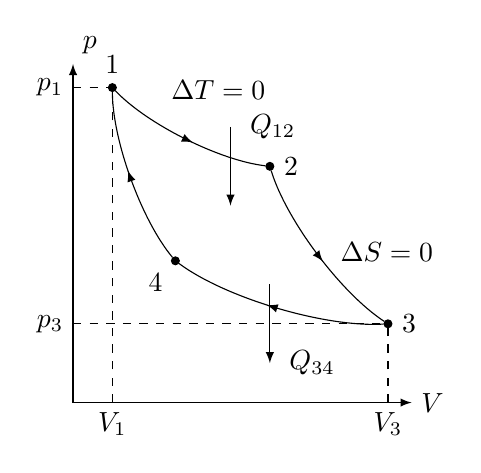
\begin{tikzpicture}[
  > = latex,
  dot/.style = {draw,fill,circle,inner sep=1pt},
  arrow inside/.style = {postaction=decorate,decoration={markings,mark=at position .55 with \arrow{>}}}
  ]
  \draw[<->] (0,4.3) node[above right] {$p$} |- (4.3,0) node[right] {$V$};
  \node[dot,label={above:$1$}] (@1) at (0.5,4) {};
  \node[dot,label={right:$2$}] (@2) at (2.5,3) {};
  \node[dot,label={right:$3$}] (@3) at (4,1) {};
  \node[dot,label={below left:$4$}] (@4) at (1.3,1.8) {};

  \node[label={above right:$\Delta T = 0$}] at (1,3.6) {};
  \node[label={above right:$\Delta S = 0$}] at (3.15,1.54) {};

  \draw[arrow inside] (@1) to[looseness=.7,bend right=20] (@2);
  \draw[arrow inside] (@2) to[looseness=.7,bend right=20] (@3);
  \draw[arrow inside] (@3) to[looseness=.7,bend left=20] (@4);
  \draw[arrow inside] (@4) to[looseness=.7,bend left=20] (@1);
  \draw[dashed,thin] (0,4) node[left] {$p_1$} -- (0.5,4);
  \draw[dashed,thin] (0,1) node[left] {$p_3$} -- (4,1);
  \draw[dashed,thin] (0.5,0) node[below] {$V_1$} -- (0.5,4);
  \draw[dashed,thin] (4,0) node[below] {$V_3$} -- (4,1);

  \draw[->] (2,3.5) to (2,2.5);
  \node[label={right:$Q_{12}$}] at (2,3.5) {};
  \draw[->] (2.5,1.5) to (2.5,0.5);
  \node[label={right:$Q_{34}$}] at (2.5,0.5) {};
\end{tikzpicture}

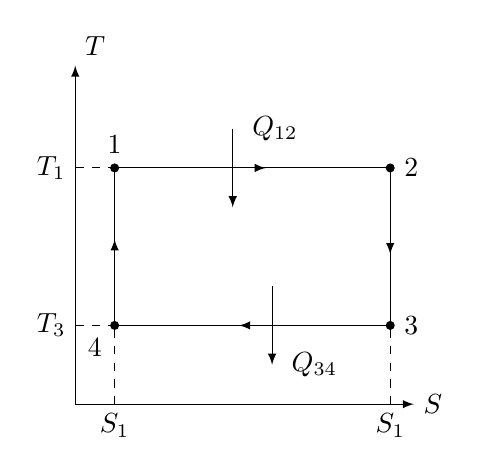
\begin{tikzpicture}[
  > = latex,
  dot/.style = {draw,fill,circle,inner sep=1pt},
  arrow inside/.style = {postaction=decorate,decoration={markings,mark=at position .55 with \arrow{>}}}
  ]
  \draw[<->] (0,4.3) node[above right] {$T$} |- (4.3,0) node[right] {$S$};
  \node[dot,label={above:$1$}] (@1) at (0.5,3) {};
  \node[dot,label={right:$2$}] (@2) at (4,3) {};
  \node[dot,label={right:$3$}] (@3) at (4,1) {};
  \node[dot,label={below left:$4$}] (@4) at (0.5,1) {};

  \draw[arrow inside] (@1) to (@2);
  \draw[arrow inside] (@2) to (@3);
  \draw[arrow inside] (@3) to (@4);
  \draw[arrow inside] (@4) to (@1);
  \draw[dashed,thin] (0,3) node[left] {$T_1$} -- (0.5,3);
  \draw[dashed,thin] (0,1) node[left] {$T_3$} -- (0.50,1);
  \draw[dashed,thin] (0.5,0) node[below] {$S_1$} -- (0.5,1);
  \draw[dashed,thin] (4,0) node[below] {$S_1$} -- (4,1);

  \draw[->] (2,3.5) to (2,2.5);
  \node[label={right:$Q_{12}$}] at (2,3.5) {};
  \draw[->] (2.5,1.5) to (2.5,0.5);
  \node[label={right:$Q_{34}$}] at (2.5,0.5) {};
\end{tikzpicture}

%   ______               _           __       
%  / ____/__  ____ ___  (_)_________/ /_  ___ 
% / / __/ _ \/ __ `__ \/ / ___/ ___/ __ \/ _ \
%/ /_/ /  __/ / / / / / (__  ) /__/ / / /  __/
%\____/\___/_/ /_/ /_/_/____/\___/_/ /_/\___/ 
%                                             
%    ____    __           __             ______              
%   /  _/___/ /__  ____ _/ /__  _____   / ____/___ _________ 
%   / // __  / _ \/ __ `/ / _ \/ ___/  / / __/ __ `/ ___/ _ \
% _/ // /_/ /  __/ /_/ / /  __/ /     / /_/ / /_/ (__  )  __/
%/___/\__,_/\___/\__,_/_/\___/_/      \____/\__,_/____/\___/ 
                                                            
\section{Gemische Idealer Gase}

\begin{align*}
	&\xi_i
	= \frac{m_i}{m}, \quad \psi_i
	= \frac{n_i}{n}, \quad p_i
	= \psi_ip \\
	&\xi_i
	= \frac{M_i n_i}{\sum_{k
	= 1}^{K} M_kn_k}
	= \frac{M_i}{M_G}\psi  
	\\
	& p_iV
	= m_iR_iT, \quad p_iV
	= n_iR_mT, \quad pV
	= mR_GT \\
	& \sum_{k
	= 1}^{K} p_k
	= p 
	\\
	&R_G
	= \frac{1}{m} \sum_{k=1}^{K} m_kR_k
	= \sum_{k=1}^{K} \xi_k R_k 
	\\
	&U_G
	= \sum_{k=1}^{K} U_k
	= \sum_{k=1}^{K} m_k u_k
	= \sum_{k=1}^{K} c_{vk}m_kT \leftarrow \text{$c_v$
	= const}
	\\
	&H_G
	= \sum_{k=1}^{K} H_k
	= \sum_{k=1}^{K} m_k h_k
	= \sum_{k=1}^{K} c_{pk}m_kT \leftarrow \text{$c_p$
	= const.}
	\\
	&c_{vG}
	= \sum_{k=1}^{K} c_{vk} \xi_k, \quad c_{pG}
	= \sum_{k=1}^{K} c_{pk}\xi_k 
	\\
	&S_2-S_1
	= R_m \left( n \ln n - \sum_{k=1}^{K} n_k \ln n_k \right)
\end{align*}

\begin{align*}
	\text{Adiabate } & \text{ Drosselung (ideal): } \\ 
	& h + \frac{c^2}{2} + gz = \text{const.} \\
	& dh = 0 \\
	\text{Adiabet } & \text{ Drosselung (real): }  \\ 
	& \delta_h = \left(\frac{\partial T}{\partial p}\right)_{h}  = - \frac{v}{c_p}(1-\beta T) \\
\end{align*}

%    _   __                    __                      ____
%   / | / /___ _______________/ /___ _____ ___  ____  / __/
%  /  |/ / __ `/ ___/ ___/ __  / __ `/ __ `__ \/ __ \/ /_  
% / /|  / /_/ (__  |__  ) /_/ / /_/ / / / / / / /_/ / __/  
%/_/ |_/\__,_/____/____/\__,_/\__,_/_/ /_/ /_/ .___/_/     
%                                           /_/            

\section{Nassdampf}
\tiny
\begin{flushleft}
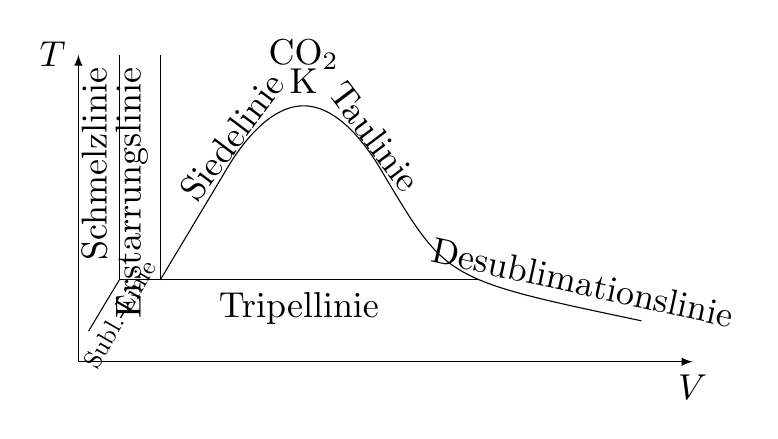
\begin{tikzpicture}
	[
	scale=1.3, every node/.style={scale=1.3},
	> = latex,
	dot/.style = {draw,fill,circle,inner sep=1pt},
	arrow inside/.style = {postaction=decorate,decoration={markings,mark=at position .55 with \arrow{>}}}
	]
	\draw[<->]  (0,3) node[left] {$T$} |- (6,0) node[below] {$V$} ;
	\draw (0.1,0.3) -- node[midway, below, rotate=60, scale=0.7] {Subl.-Linie} (0.4,0.8);
	\draw (0.4, 0.8) -- (0.4, 3) node[above left, rotate=90] {Schmelzlinie};
	\draw (0.8, 0.8) -- (0.8, 3) node[above left, rotate=90] {Erstarrungslinie};
	\draw (0.4,0.8) -- node[midway, below] {Tripellinie} (3.91,0.8);
	\draw (0.8,0.8) -- (1.4,1.8);
	\draw (1.4,1.8) parabola bend (2.2,2.5) (3,1.8);
	\draw (3,1.8)  .. controls (3.6,0.8) .. node[very near end, sloped, above] {Desublimationslinie} (5.5,0.4);
	\draw (1.5,2.2) node[rotate=53] {Siedelinie};
	\draw (2.9,2.2) node[rotate=-53] {Taulinie};
	\draw (2.2,3) node {$\text{CO}_\text{2}$};
	\draw (2.2,2.5) node[above] {K};
\end{tikzpicture}

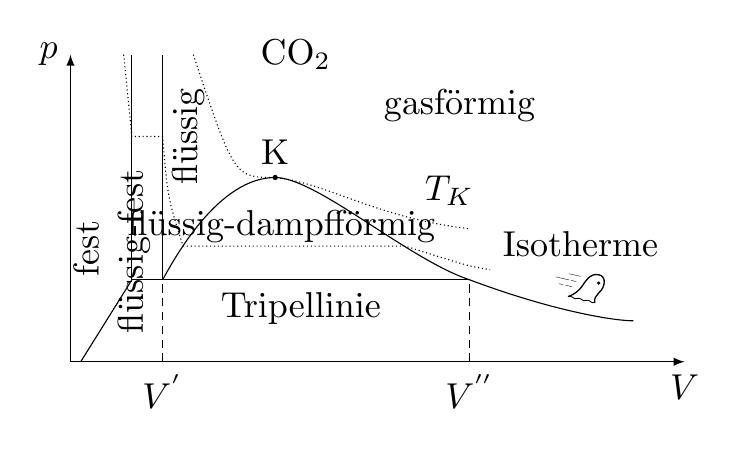
\begin{tikzpicture}
	[
	scale=1.3, every node/.style={scale=1.3},
	> = latex,
	dot/.style = {draw,fill,circle,inner sep=1pt},
	arrow inside/.style = {postaction=decorate,decoration={markings,mark=at position .55 with \arrow{>}}}
	]
	\draw[<->]  (0,3) node[left] {$p$} |- (6,0) node[below] {$V$} ;
	\draw (0.1,0) -- (0.6,0.8);
	\draw (0.6, 0.8) -- (0.6, 3) ;
	\draw (0.9, 0.8) -- (0.9, 3);
	\draw (0.6,0.8) -- node[midway, below] {Tripellinie} (3.9,0.8);

	\draw (0.9,0.8) parabola[bend at end]  (2, 1.8);

	\draw (2,1.8) .. controls (2.4,1.8) and (3.3, 1) .. (3.9,0.8) .. controls (4.7,0.5) and (5.3,0.4) .. node[above, sloped]  {$\xrightswishingghost{}$} (5.5,0.4);
	\draw (2.2,3) node {$\text{CO}_\text{2}$};

	\draw[fill] (2,1.8) circle (0.02) node[above] {K};

	\draw[densely dashed] (0.9,0) node[below] {$V^{'}$} -- (0.9,0.8);
	\draw[densely dashed] (3.9,0) node[below] {$V^{''}$} -- (3.9,0.8);
	\draw (3.7,1.4) node[above]  {$T_K$};
	\draw (0.4,1.5) node[above left, rotate=90] {fest};
	\draw (1.15,2.2) node[rotate=90] {flüssig};
 	\draw (0.9,2) node[above left, rotate=90] {flüssig-fest};
	\draw (2.06,1.32) node {flüssig-dampfförmig};
	\draw (3.8,2.5) node {gasförmig};

	\draw[densely dotted] (1.2,3) ..controls (1.6,1.8) .. (2,1.8) .. controls(2.5,1.75) and (3,1.4) .. (3.9, 1.3);
	\draw[densely dotted] (0.52,3) to (0.6,2.2) to (0.6,2.2) to (0.9,2.2) .. controls (0.95,1.6) .. (1.1,1.13) -- (3.27,1.13) .. controls (3.9,0.93) .. (4.1,0.9) node[above right] {Isotherme};
\end{tikzpicture}

%\small
%\begin{tikzpicture}
%	 [> = latex,
%	dot/.style = {draw,fill,circle,inner sep=1pt},
%	arrow inside/.style = {postaction=decorate,decoration={markings,mark=at position .55 with \arrow{>}}}
%	]
%	\draw[<->]  (0,3) node[left] {$p$} |- (3.5,0) node[below] {$v$};
%	\draw (1,1.8) parabola bend (1.5,2.4) (2,1.8);
%	\draw (0.4,0.3) -- (1,1.8);
%	\draw (2,1.8) to[bend right=10] (3,0.3);
%\end{tikzpicture}

\end{flushleft}
\normalsize
\begin{multicols}{2}

\begin{align*}
	& v = (1-x)v^{'} + xv{''} \\
	& v = v^{'} + (v^{''}-v^{'})x \\ \\
	& u = (1-x) u^{'} + xu^{''} \\
	& u = u^{'} + (u^{''}-u^{'})x \\ \\
	& h = (1-x) h^{'} + xh^{''} \\
	& h = h^{'} + (h^{''}-h^{'})x \\ \\
	& s = (1-x) s^{'} + xs^{''} \\
	& s = s^{'} + (s^{''}-s^{'})x \\ \\
	& r = h^{''} - h^{'} = T(s^{''}-s^{'}) \\
\end{align*}

\begin{align*}
	& T^{'} = T^{''} \\
	& p^{'} = p^{''} \\
	& g^{'} = g^{''} \\
	&dg^{'} = v^{'}dp^{'} - s^{'}dT^{'} \\
	&dg^{''} = v^{''} dp^{''} - s^{''} dT^{''} \\
	&dg^{'} = dg^{''} \\
	& \frac{dp}{dT} = \frac{s^{''} - s^{'}}{v^{''} - v^{'}} \\
	& \frac{dp}{dT} = \frac{1}{T}\frac{h^{''} - h^{'}}{v^{''} - v^{'}} \\
	& \frac{dp}{dT} = \frac{1}{T}\frac{r}{v^{''} -v^{'}} \\
\end{align*}
\end{multicols}

%    ____             __             _____ __        ________   _         
%   / __ \___  ____ _/ /__  _____   / ___// /_____  / __/ __/  (_)___ ___ 
%  / /_/ / _ \/ __ `/ / _ \/ ___/   \__ \/ __/ __ \/ /_/ /_   / / __ `__ \
% / _, _/  __/ /_/ / /  __/ /      ___/ / /_/ /_/ / __/ __/  / / / / / / /
%/_/ |_|\___/\__,_/_/\___/_/      /____/\__/\____/_/ /_/    /_/_/ /_/ /_/ 
%                                                                         
%    _   __                    __                      ____           __    _      __
%   / | / /___ _______________/ /___ _____ ___  ____  / __/___  ___  / /_  (_)__  / /
%  /  |/ / __ `/ ___/ ___/ __  / __ `/ __ `__ \/ __ \/ /_/ __ `/ _ \/ __ \/ / _ \/ _/
% / /|  / /_/ (__  |__  ) /_/ / /_/ / / / / / / /_/ / __/ /_/ /  __/ /_/ / /  __/ /__
%/_/ |_/\__,_/____/____/\__,_/\__,_/_/ /_/ /_/ .___/_/  \__, /\___/_.___/_/\ __/\___/
%                                           /_/        /____/                 

\section{Realer Stoff im Nassdampfgebiet}
\begin{align*}
	\text{Isobare } &\text{Zustandsänderung} \\
	q_{12} &= T(s_2 - s_1) \\
	&= T\Big(s^{''} - s^{'}\Big)(x_2-x_1) \\
	w_{V,12} &= - \int_{1}^{2} p\; dv \\
	&= -p(v_2-v_1) = -p\Big(v^{''} -v^{'}\Big)(x_2-x_1) \\
	\text{Isochore } &\text{Zustandsänderung} \\
	q_{12} &= u_2 - u_1 = u_2^{'} + x_2\Big(u_2^{''} - u_2^{'} \Big) - u_1^{'} - x_1\Big(u_1^{''} - u_1^{'}\Big) \\
	\text{Adiabate } &\text{Zustandsänderung} \\
	w_{V,12} &= u_2 - u_1 = u_2^{'} + x_2 \Big( u_2^{''} - u_2^{'} \Big) - u_1^{'} - x_1\Big(u_1^{''} - u_1^{'}\Big) \\
	\text{Entropie} & \text{änderung wärend des Mischvorgangs} \\
	&S_2-S_2 = R_m \left ( n \ln n - \sum_{i}^{} n_i \ln n_i \right ) \\
\end{align*}

%    ______                     _    
%   / ____/  _____  _________ _(_)__ 
%  / __/ | |/_/ _ \/ ___/ __ `/ / _ \
% / /____>  </  __/ /  / /_/ / /  __/
%/_____/_/|_|\___/_/   \__, /_/\___/ 
%	              /____/         

\section{Maximale Arbeit und Exergie}
Maxiaml nutzbare Arbeit $\rightarrow$ isentrop, reibungsfrei \\
$1 \rightarrow 1'$ : isentrop auf $T_u$ \\
$1' \rightarrow u$ : isotherm auf $u$ 

\begin{multicols}{2}


	\begin{flushleft}

\begin{tikzpicture}[
	scale=0.8, every node/.style={scale=1},
  > = latex,
  dot/.style = {draw,fill,circle,inner sep=1pt},
  arrow inside/.style = {postaction=decorate,decoration={markings,mark=at position .55 with \arrow{>}}}
  ]
  	\draw[<->] (0,4.3) node[above right] {$T$} |- (4.3,0) node[right] {$S$};

	\coordinate (a) at (0.8,0.6);
	\coordinate (b) at (0.8,2);

	\coordinate (c) at (3.3,3.5);
	\coordinate (d) at (3.3,2);

	\coordinate (u) at (2,2);
	\node[dot,label={above left:$u$}] at (u) {};

	\node[dot,label={below left:$1$}] at (a) {};
	\node[dot,label={above left:$1'$}] at (b) {};

  	\draw[thick, arrow inside] (a) to (b);
  	\draw[thick, arrow inside] (b) to (u);

	\node[dot,label={below left:$2$}] at (c) {};
	\node[dot,label={above left:$2'$}] at (d) {};

  	\draw[thick, arrow inside] (c) to (d);
  	\draw[thick, arrow inside] (d) to (u);

  	\draw[dashed,thin] (0,2) node[left] {$T_u$} -- (2,2);
  	\draw[dashed,thin] (2,0) node[below] {$S_u$} -- (2,2);

\end{tikzpicture}
\end{flushleft}
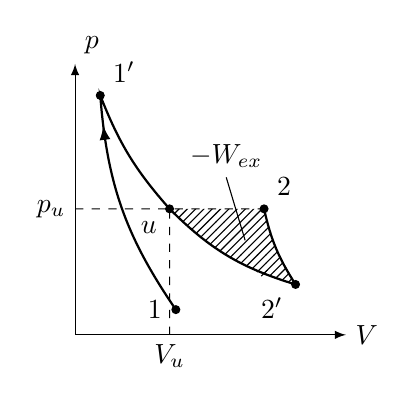
\begin{tikzpicture}[
	scale=0.8, every node/.style={scale=1},
  > = latex,
  dot/.style = {draw,fill,circle,inner sep=1pt},
  arrow inside/.style = {postaction=decorate,decoration={markings,mark=at position .55 with \arrow{>}}}
  ]
  \draw[<->] (0,4.3) node[above right] {$p$} |- (4.3,0) node[right] {$V$};
	\coordinate (a) at (1.6,0.4);
	\coordinate (b) at (0.4,3.8);

	\coordinate (c) at (3,2);
	\coordinate (d) at (3.5,0.8);

	\coordinate (u) at (1.5,2);
	\node[dot,label={below left:$u$}] at (u) {};

	\node[dot,label={left:$1$}] at (a) {};
	\node[dot,label={above right:$1'$}] at (b) {};

	\draw[thick, arrow inside] (a) to[bend left=15] (b) to[bend right=10] (u);

	\node[dot,label={above right:$2$}] at (c) {};
	\node[dot,label={below left:$2'$}] at (d) {};

	\draw[thick, arrow inside, pattern=north east lines] (c) to[bend right=10] (d) to[bend left=14] (u);
	\draw (2.7,1.5) to (2.4,2.5) node[above] {$-W_{ex}$};

  	\draw[dashed,thin] (0,2) node[left] {$p_u$} -- (c);
  	\draw[dashed,thin] (1.5,0) node[below] {$V_u$} -- (u);
\end{tikzpicture}
\end{multicols}

\begin{multline*}
	-\dot{W}_{ex} = - (\dot{W}_t)_{rev} = -\frac{d}{dt} \left( U + m\left ( \frac{c^2}{2}+ gz \right) + p_uV - T_uS \right) \\  +  \sum_{j=1}^{K} \left(\dot{m}_j \left(h + \frac{c^2}{2} + gz -T_s \right) \right) + \sum_{l=1}^{K} \left( 1 - \frac{T_u}{T}\right) \dot{Q}_l 
\end{multline*}


Die Exergie der Enthalpie (offens, stationäres System)
\begin{equation*}
	-\dot{W}_{ex,1u} = \dot{m}(h_1 - h_u -T_u(s_1 - s_u))
\end{equation*}
Die Exergie der inneren Energie (geschlossenes, instationäres System)
\begin{align*}
	- \dot{W}_{ex} &= - \frac{d}{dt}(U + p_uV -T_uS) \\
	-\dot{W}_{ex,1u} &= U_1 - U_u -p_u(V_1 - V_u) - T_u(S_1 - S_u) \\
	-\dot{W}_{ex,1u} &= H_1 - (p_1-p_u)V_1 - H_u- T_u(S_1 - S_u)
\end{align*}
Für Ideales Gas \\
\begin{align*}
	-W_{ex} = mc_v(T_1 -T_u) + p_u(V_1 - V_u) - T_um \left(c_p \ln \left(\frac{T_1}{T_u}\right) -R_i \ln \left(\frac{p_1}{p_u}\right)\right)
\end{align*}
Dampf/Luftdruckkammer
\begin{equation*}
	-W_{ex,1u} = m_1 [ u_1 - u_u + p_u ( v_1 - v_u) - T_u(s_1 - s_u)]
\end{equation*}
Die Exergie der Wärme (geschlossenes, stationäres System)
\begin{equation*}
	- \dot{W}_{ex} = \left(1 - \frac{T_u}{T_1} \right) \dot{Q}_1 = \eta_{th,C} \dot{Q}_1 \\
\end{equation*}

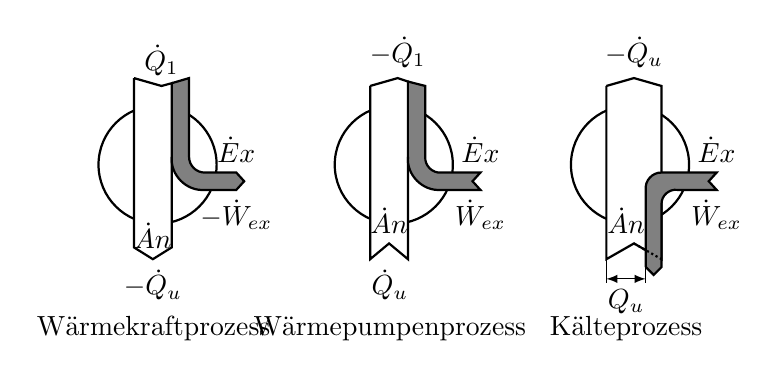
\begin{tikzpicture}[
		\thicc,
		scale=1, every node/.style={scale=1},
  		> = latex,
  		dot/.style = {draw,fill,circle,inner sep=1pt},
  		arrow inside/.style = {postaction=decorate,decoration={markings,mark=at position .55 with \arrow{>}}}
		]

	\draw 	(1,1.2) node [minimum size=1.5cm,circle,draw] {};

	\coordinate (a1) at (0.7,2.3);
	\coordinate (a2) at (1.05,2.2);
	\coordinate (a3) at (1.18,2.235);
	\coordinate (a4) at (1.18,0.15);
	\coordinate (a5) at (0.94,0);
	\coordinate (a6) at (0.7,0.15);
	\coordinate (a7) at (1.4,2.3);
	\coordinate (a8) at (1.4,1.3);
	\coordinate (a9) at (1.6,1.1);
	\coordinate (a10) at (2,1.1);
	\coordinate (a11) at (2.1,0.99);
	\coordinate (a12) at (2,0.88);
	\coordinate (a13) at (1.6,0.88);
	\coordinate (a14) at (1.18,1.3);
	
	\draw[fill=white] 	(a1) to (a2) to (a3) to (a4) to (a5) to (a6) to (a1);
	\draw[fill=gray] 	(a3) to (a7) to (a8) to[bend right=45] (a9) to (a10) to (a11) to (a12) to (a13) to[bend left=50] (a14);
	\draw (a3) to (a4);

	\draw 	(a2) node[above] {$\dot{Q}_1$};
	\draw 	(a5) node[above] {$\dot{A}n$};
	\draw 	(a5) node[below] {$-\dot{Q}_u$};
	\draw 	(a10) node[above] {$\dot{E}x$};
	\draw 	(a12) node[below] {$-\dot{W}_{ex}$};

	\draw (0.95,-0.6) node[below] {Wärmekraftprozess};


	\draw 	(4,1.2) node [minimum size=1.5cm,circle,draw] {};

	\coordinate (b1) at (3.7,2.2);
	\coordinate (b2) at (4.05,2.3);
	\coordinate (b3) at (4.18,2.256);
	\coordinate (b4) at (4.18,0);
	\coordinate (b5) at (3.94,0.2);
	\coordinate (b6) at (3.7,0.0);
	\coordinate (b7) at (4.4,2.2);
	\coordinate (b8) at (4.4,1.3);
	\coordinate (b9) at (4.6,1.1);
	\coordinate (b10) at (5.1,1.1);
	\coordinate (b11) at (5,0.99);
	\coordinate (b12) at (5.1,0.88);
	\coordinate (b13) at (4.6,0.88);
	\coordinate (b14) at (4.18,1.3);

	\draw[fill=white] 	(b1) to (b2) to (b3) to (b4) to (b5) to (b6) to (b1);
	\draw[fill=gray] 	(b3) to (b7) to (b8) to[bend right=50] (b9) to (b10) to (b11) to (b12) to (b13) to[bend left=50] (b14);
	\draw (b3) to (b4);

	\draw 	(b2) node[above] {$-\dot{Q}_1$};
	\draw 	(b5) node[above] {$\dot{A}n$};
	\draw 	(3.95,0) node[below] {$\dot{Q}_u$};
	\draw 	(b10) node[above] {$\dot{E}x$};
	\draw 	(b12) node[below] {$\dot{W}_{ex}$};

	\draw (3.95,-0.6) node[below] {Wärmepumpenprozess};


	\draw 	(7,1.2) node [minimum size=1.5cm,circle,draw] {};

	\coordinate (c1) at (6.7,2.2);
	\coordinate (c2) at (7.05,2.3);
	\coordinate (c3) at (7.4,2.2);
	\coordinate (c4) at (7.4,0);
	\coordinate (c5) at (7.05,0.2);
	\coordinate (c6) at (6.7,0.0);
	\coordinate (c7) at (7.2,-0.1);
	\coordinate (c8) at (7.2,0.88);
	\coordinate (c9) at (7.4,1.1);
	\coordinate (c10) at (8.1,1.1);
	\coordinate (c11) at (8,0.99);
	\coordinate (c12) at (8.1,0.88);
	\coordinate (c13) at (7.6,0.88);
	\coordinate (c14) at (7.4,0.70);
	\coordinate (c15) at (7.4,-0.1);
	\coordinate (c16) at (7.3,-0.2);

	\draw[fill=white] 	(c1) to (c2) to (c3) to (c4) to (c5) to (c6) to (c1);
	\draw[fill=gray] 	(c8)  to (c7)  to (c8)  to[bend left=50] (c9)  to (c10)  to (c11)  to (c12)  to (c13)  to[bend right=50] (c14)  to (c15) to (c16) to (c7);

	\draw 	(c2) node[above] {$-\dot{Q}_u$};
	\draw 	(6.95,0.2) node[above] {$\dot{A}n$};
	\draw 	(c10) node[above] {$\dot{E}x$};
	\draw 	(c12) node[below] {$\dot{W}_{ex}$};
	\draw[densely dotted] (c5) to (c4);
	\draw[thin] (c6) to (6.7,-0.3);
	\draw[thin] (c7) to (7.2,-0.3);
	\draw[thin,<->] (6.7,-0.25) to (7.2,-0.25);
	\draw (6.95,-0.25) node[below] {$Q_u$};

	\draw (6.95,-0.6) node[below] {Kälteprozess};
\end{tikzpicture}

                   
% _       __ /\// /|___/|                   __                           _ __   /\// /|___/|_ 
%| |     / ///\/ | __  /________ ___  ___  / /______ _____  ____ _____  (_) /__//\/ | __  / /_
%| | /| / / _ | / /_/ / ___/ __ `__ \/ _ \/ //_/ __ `/ __ \/ __ `/_  / / / __/ _ | / /_/ / __/
%| |/ |/ / __ |/___  / /  / / / / / /  __/ ,< / /_/ / /_/ / /_/ / / /_/ / /_/ __ |/___  / /_  
%|__/|__/_/ |_|/   |/_/  /_/ /_/ /_/\___/_/|_|\__,_/ .___/\__,_/ /___/_/\__/_/ |_|/   |/\__/  
%                                                 /_/                                         
\section{Wärmekapazität}

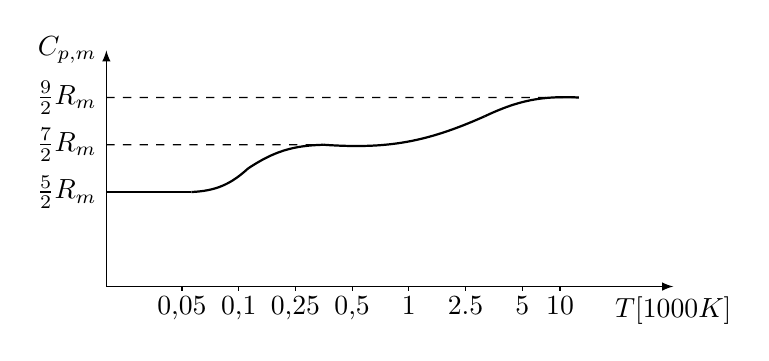
\begin{tikzpicture}[
	scale=1.2, every node/.style={scale=1},
  > = latex,
  dot/.style = {draw,fill,circle,inner sep=1pt},
  arrow inside/.style = {postaction=decorate,decoration={markings,mark=at position .55 with \arrow{>}}}
  ]
	\draw[<->] (0,2.5) node[left] {$C_{p,m}$} |- (6,0) node[below] {$T[1000K]$};

	\coordinate (a) at (0,1);
	\coordinate (b) at (0.9,1);
	\coordinate (c) at (1.5,1.25);
	\coordinate (d) at (2.3,1.5);
	\coordinate (e) at (4,1.8);
	\coordinate (f) at (5,2);
	
	\coordinate (g) at (0.8,0);
	\coordinate (h) at (1.4,0);
	\coordinate (i) at (2.0,0);
	\coordinate (j) at (2.6,0);
	\coordinate (k) at (3.2,0);
	\coordinate (l) at (3.8,0);
	\coordinate (m) at (4.4,0);
	\coordinate (n) at (4.8,0);

	\draw[dashed] (0,2) node[left] {$\frac{9}{2}R_m$} -- (f);
	\draw[dashed] (0,1.5) node[left] {$\frac{7}{2}R_m$} -- (d);
	\draw (a) node[left] {$\frac{5}{2}R_m$};

	\draw[thick] (a) to (b);
	\draw[thick] (b) to[bend right=20] (c);
	\draw[thick] (c) to[bend left=16] (d);
	\draw[thick] (d) to[bend right=14] (e);
	\draw[thick] (e) to[bend left=14] (f);

	\draw (g) node[below] {0,05} to ($ (g) - (0,0.05) $);
	\draw (h) node[below] {0,1} to ($ (h) - (0,0.05) $);
	\draw (i) node[below] {0,25} to ($ (i) - (0,0.05) $);
	\draw (j) node[below] {0,5} to ($ (j) - (0,0.05) $);
	\draw (k) node[below] {1} to ($ (k) - (0,0.05) $);
	\draw (l) node[below] {2.5} to ($ (l) - (0,0.05) $);
	\draw (m) node[below] {5} to ($ (m) - (0,0.05) $);
	\draw (n) node[below] {10} to ($ (n) - (0,0.05) $);
\end{tikzpicture}

\begin{align*}
	&	C_{v,m} = \frac{1}{\kappa - 1} R_m
		&&C_{p,m} = \frac{\kappa}{\kappa -1}r_m \\
	&	c_v = \frac{1}{\kappa - 1 }R_j 
		&&c_p = \frac{\kappa}{\kappa -1}R_j \\
	&	\kappa = \frac{c_p}{c_v}
	&&R = c_p - c_v \\
	&R = \frac{R_m}{M}
	&&R_m = 8,3143\left[\frac{kJ}{kmolK}\right] \\
	\end{align*}
	\begin{multline*}
		C_{v,m} = \underbrace{3 + \frac{R_m}{2}}_{\text{Translatorisch}} + \underbrace{\frac{n_{\text{rot}}  R_m}{2}}_{\text{Rotatorisch}}  
		+ \underbrace{R_M ( 3n_{\text{Atome}} - 3 - n_{rot})}_{\text{Vibratorisch}}  \\
		+ \underbrace{C_{v,m,Elektronenanregung}}_{\text{Relevant ab: }T \approx 10^4K } 
	\end{multline*}
%  ______          __          _           __       
% /_  __/__  _____/ /_  ____  (_)_________/ /_  ___ 
%  / / / _ \/ ___/ __ \/ __ \/ / ___/ ___/ __ \/ _ \
% / / /  __/ /__/ / / / / / / (__  ) /__/ / / /  __/
%/_/  \___/\___/_/ /_/_/ /_/_/____/\___/_/ /_/\___/ 
%                                                         
%    ___                                 __                 
%   /   |  ____ _      _____  ____  ____/ /_  ______  ____ _
%  / /| | / __ \ | /| / / _ \/ __ \/ __  / / / / __ \/ __ `/
% / ___ |/ / / / |/ |/ /  __/ / / / /_/ / /_/ / / / / /_/ / 
%/_/  |_/_/ /_/|__/|__/\___/_/ /_/\__,_/\__,_/_/ /_/\__, /  
%                                                  /____/   

\onecolumn
\section{Technische Anwendung}

\begin{centering}
\begin{tabular}{lll} 
	\begin{tabular}{l}
	adiabat \\ $(c_p = const.)$
	\end{tabular}
	& $ \displaystyle W_{t,12} = mc_p(T_2 - T_1) = \frac{\kappa}{\kappa -1}(p_2V_2 - p_1V_1)$ & $Q_{12}=0$\\ \hline
	\begin{tabular}{l}
	reversibel adiabat \\ 
	$ \kappa = const.$
	\end{tabular}
	& $\displaystyle W_{t,12} = \frac{\kappa}{\kappa -1} (p_1 V_1)\left[\left(\frac{p_2}{p_1}\right)^{\frac{\kappa - 1}{\kappa}} - 1 \right]$ & $Q_{12}=0$ \\ \hline
	\begin{tabular}{l}
	irreversibel adiabat \\ 
	als Polytrope \\ 
	$n>\kappa; n,\kappa = const.$
	\end{tabular}
	& $\displaystyle W_{t,12} = \frac{\kappa}{\kappa -1} (p_1 V_1)\left[\left(\frac{p_2}{p_1}\right)^{\frac{n - 1}{n}} - 1 \right]$ & $Q_{12}=0$ \\ \hline
	\begin{tabular}{l}
	reversibel polytrop \\ $n,\kappa = const.$ 
	\end{tabular}
		& $W_{t,12} = \frac{n}{n-1}(p_2V_2 - p_1V_1)$ & $Q_{12} = mc_n(T_2-T_1)$ \\
	 & $\qquad \: = \frac{n}{n-1}mR(T_2-T_1)$ &  $\quad \;\;\; =\frac{n-\kappa}{(n-1)(\kappa-1)}(p_1V_1) \left[ \left( \frac{p_2}{p_1}\right)^{\frac{n-1}{n} - 1}\right]$ \\
	 & $\qquad \: = \frac{n}{n-1}(p_1V_1) \left[\left( \frac{p_2}{p_1}\right)^{\frac{n-1}{n}} - 1 \right]$ & $ c_n \;\; = \frac{n-\kappa}{n-1}cv$\\ \hline
	 isotherm & $ W_{t,12} = (p_1V_1) \ln \left(\frac{p_2}{p_2}\right)$ & $Q_{12} = -W_{t,12}$ \\
\end{tabular}
\end{centering}
\bigskip

\begin{tabular}{lllll}
	Thermischer Wirkungsgrad 
	&
	$\eta_{th}$ & $\displaystyle = \frac{-w}{q_{zu}} = \frac{\text{Nutzen}}{\text{Aufwand}}$ &$= \displaystyle 1 - \frac{|q_{ab}|}{q_{zu}}$ &
	\multirow{2}{*}{
	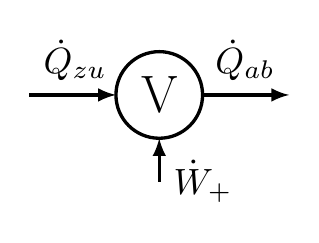
\begin{tikzpicture}
		[remember picture, 
		very thick,
		scale=1, every node/.style={scale=1.1},
  		> = latex,
  		dot/.style = {draw,fill,circle,inner sep=1pt},
  		arrow inside/.style = {postaction=decorate,decoration={markings,mark=at position .55 with \arrow{>}}}
		]
		\pic (B) {verdichter};
	\end{tikzpicture}}
	\\\\
	Isentroper Verdichterwirkungsgrad
	& 
	$\eta_{sV}$ & $\displaystyle = \frac{w_{t,12,rev}}{w_{t,12}}$ &$\displaystyle =\frac{h_{2,rev} - h_1}{h_2 - h_1}$ \\\\
	Isentroper  Turbinenwirkungsgrad 
	&
	$\eta_{sT}$ & $\displaystyle = \frac{w_{t,12}}{W_{t,12,rev}}$ & $ \displaystyle = \frac{h_1 - h_2}{h_1 - h_{2,rev}}$ &
	\multirow{2}{*}{
	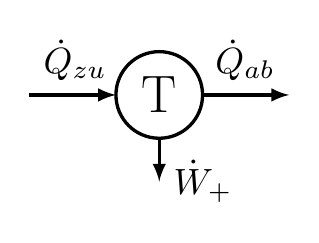
\begin{tikzpicture}
		[remember picture,
		very thick,
		scale=1, every node/.style={scale=1.1},
  		> = latex,
  		dot/.style = {draw,fill,circle,inner sep=1pt},
  		arrow inside/.style = {postaction=decorate,decoration={markings,mark=at position .55 with \arrow{>}}}
		]
		\pic (A) {turbine};
	\end{tikzpicture}}
	\\\\
	Dampfkraftprozess Wirkungsgrad 
	&
	$n_{th}$ &$\displaystyle = 1 - \frac{|q_{61}|}{q_{23}+q{34} + q_{45}}$ 
	& 
	$\displaystyle = 1 - \frac{h_6 - h_1}{h_5 -  h_2}$ \\\\
	Leistungszahl Kältemaschine &
	$\epsilon_{K(A)}$ &$\displaystyle = \frac{q_{zu}}{w} = \frac{\dot{Q}_0}{\dot{W}}$ \\\\
	Leistungszahl Kaltluftprozess &
	$\epsilon_{K}$ &$\displaystyle = \frac{1}{\left(\frac{p}{p_0}\right)^{\frac{\kappa - 1}{\kappa} - 1}}$ \\\\
	Leistungszahl Kaltdampfprozess &
	$\epsilon_K$ & $\displaystyle = \frac{q_0}{|q| - q_0} = \frac{q_o}{w_t}$ &$\displaystyle = \frac{h_1 - h_6}{h_2 - h_1}$ \\\\
	Linkslaufender Carnotprozess &
	$\epsilon_{carnot}$ &$\displaystyle = \frac{T_k}{T_H-T_K}$ \\
	Leistungszahl Wärmepumpe &
	$\epsilon_{WP}$ & $\displaystyle = \frac{q}{|q| - q_0} = \frac{|q|}{w_t} = \frac{q_{zu}}{w}$ &$\displaystyle = \frac{h_2 - h_5}{h_2 - h_1} = 1 + \epsilon_{K(A)}$ \\\\
	Verdichtungsverhältnis &
	$\epsilon$ &$\displaystyle = \frac{v_1}{v_2}$ \\\\
	Drucksteigerungsverhältniss &
	$\psi$ &$\displaystyle = \frac{p_3}{p_2}$ \\\\
	Einspriztverhältniss &
	$\varphi $ &$\displaystyle = \frac{v_4}{v_3}$ \\\\
	Temperaturverhältnis &
	$\tau$ &$ \displaystyle \displaystyle =\frac{T_3}{T_1}$ \\\\
	Verdrichtungsdruckverhältnis &
	$\pi$ = & $ \displaystyle  = \frac{p_2}{p_1}$ \\\\
	für Joule-Prozess &
	$\pi_{opt}$ & $ \displaystyle = \tau^{\frac{\kappa}{2(\kappa -1)}}$ \\
	
	
\end{tabular}

\pagebreak

%\begin{tikzpicture}[
%		thick,
%		scale=1, every node/.style={scale=1},
%  		> = latex,
%  		dot/.style = {draw,fill,circle,inner sep=1pt},
%  		arrow inside/.style = {postaction=decorate,decoration={markings,mark=at position .55 with \arrow{>}}}
%		]
%
%	\draw 	(1,1) node [minimum size=1cm,circle,draw] {\LARGE T};
%
%	\draw[->] (-0.5,1) node[above right] {$\dot{Q}_{zu}$} to (0.5,1);
%	\draw[->] (1.5,1)  to (2.5,1) node[above left] {$\dot{Q}_{ab}$};
%	\draw[->] (1,0) node[right] {$\dot{W}_+$} to (1,0.5);
%
%	\draw (0.95,-0.6) node[below] {Turbine};
%
%
%	\draw 	(8,1) node [minimum size=1cm,circle,draw] {\LARGE V};
%
%	\draw[->] (6.5,1) node[above right] {$\dot{Q}_{zu}$} to (7.5,1);
%	\draw[->] (8.5,1)  to (9.5,1) node[above left] {$\dot{Q}_{ab}$};
%	\draw[<-] (8,0) node[right] {$\dot{W}_+$} to (8,0.5);
%
%	\draw (7.95,-0.6) node[below] {Verdichter};
%	
%\end{tikzpicture}

\subsection*{Kolbenverdichter}

\begin{multicols}{2}

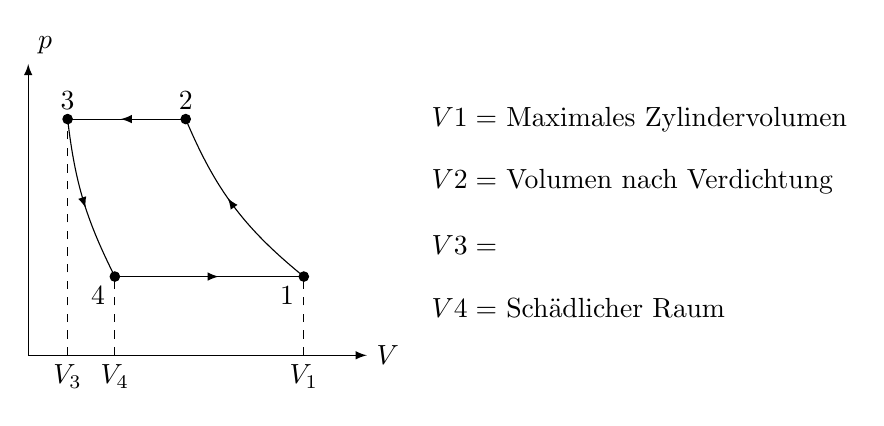
\begin{tikzpicture}[
	%\thicc,
  	> = latex,
  	dot/.style = {draw,fill,circle,inner sep=1pt},
  	arrow inside/.style = {postaction=decorate,decoration={markings,mark=at position .55 with \arrow{>}}}
  	]

  	\draw[<->] (0,3.7) node[above right] {$p$} |- (4.3,0) node[right] {$V$};

  	\coordinate (@1) at (3.5,1);
  	\coordinate (@2) at (2,3);
  	\coordinate (@3) at (0.5,3);
  	\coordinate (@4) at (1.1,1);

	\draw[fill] (@1) circle (0.06) node[below left] {1};
	\draw[fill] (@2) circle (0.06) node[above] {2};
	\draw[fill] (@3) circle (0.06) node[above] {3};
	\draw[fill] (@4) circle (0.06) node[below left] {4};
	

	\draw[arrow inside] (@1) to[bend left=14] (@2);
 	\draw[arrow inside] (@2) to (@3);
	\draw[arrow inside] (@3) to[bend right=10] (@4);
 	\draw[arrow inside] (@4) to (@1);
	
  	\draw[dashed,thin] (3.5,0) node[below] {$V_1$} -- (@1);
  	\draw[dashed,thin] (0.5,0) node[below] {$V_3$} -- (@3);
  	\draw[dashed,thin] (1.1,0) node[below] {$V_4$} -- (@4);
	
	\draw (5,3.0) node[right] {$V1 =$ Maximales Zylindervolumen};
	\draw (5,2.2) node[right] {$V2 =$ Volumen nach Verdichtung};
	\draw (5,1.4) node[right] {$V3 =$ };
	\draw (5,0.6) node[right] {$V4 =$ Schädlicher Raum};
	
\end{tikzpicture}


\begin{alignat*}{2}
	\mu &= \frac{V_1 - V_4}{V_1-V3}, \qquad \epsilon_S = \frac{V_3}{V_1 - V_3} \\
	\mu &= 1 - \epsilon_S \left[\left(\frac{p_2}{p_1}\right)^{\frac{1}{n}} -1 \right] \\
	W_{t,12} & = \int_{1}^{2} V\; dp \\
	&=\underbrace{p_2 V_2}_{Ausschiebearbeit} - \underbrace{p_1 V_1}_{Einschiebearbeit} - \int_{1}^{2} p\; dV	\\
	&= \frac{n}{n-1}p_1(V_1-V_4) \left[\left(\frac{p_2}{p_1}\right)^{\frac{n-1}{n}} - \right] \\
\end{alignat*}

\end{multicols}


%  ______           __                             ___      __    __           
% /_  __/_  _______/ /_  ____ _   _____  _________/ (_)____/ /_  / /____  _____
%  / / / / / / ___/ __ \/ __ \ | / / _ \/ ___/ __  / / ___/ __ \/ __/ _ \/ ___/
% / / / /_/ / /  / /_/ / /_/ / |/ /  __/ /  / /_/ / / /__/ / / / /_/  __/ /    
%/_/  \__,_/_/  /_.___/\____/|___/\___/_/   \__,_/_/\___/_/ /_/\__/\___/_/     
%                                                                              
\subsection*{Turboverdichter}
\begin{multicols}{2}

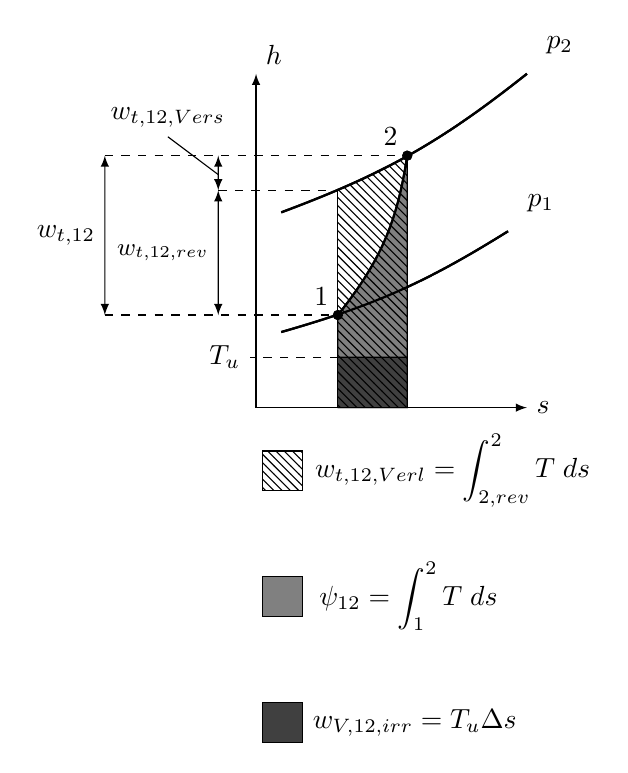
\begin{tikzpicture}[
	scale=0.8, every node/.style={scale=1},
  > = latex,
  dot/.style = {draw,fill,circle,inner sep=1pt},
  arrow inside/.style = {postaction=decorate,decoration={markings,mark=at position .55 with \arrow{>}}}
  ]
  	\draw[<->] (0,5.3) node[above right] {$h$} |- (4.3,0) node[right] {$s$};

	\coordinate (@1) at (0.4,1.2);
	\coordinate (@2) at (4,2.8);
	\coordinate (@3) at (0.4,3.1);
	\coordinate (@4) at (4.3,5.3);
	\coordinate (@5) at (1.3,0);
	\coordinate (@6) at (1.3,3.45);
	\coordinate (@7) at (-0.6,3.45);
	\coordinate (@8) at (-2.4,1.470);
	\coordinate (@9) at (1.3,1.470);
	\coordinate (@10) at (-2.4,4);
	\coordinate (@11) at (2.4,4);
	\coordinate (@12) at (2.4,0);

	\node[label={above right:$p_1$}] at (@2) {};
	\node[label={above right:$p_2$}] at (@4) {};

	\draw[thick] (@1) to[bend right=8] (@2);
	\draw[thick] (@3) to[bend right=9] (@4);
	\draw[thick] (@9) node[dot] {} to[bend right=15] (@11) node[dot] {};
	\draw[fill=gray] (@9) to (@5) to (@12) to (@11) to[bend left=15] (@9);
	\draw[fill=darkgray] (@5) to (@12) to (2.4,0.8) to (1.3,0.8);
	\draw[pattern=north west lines] (@6) to (@5) to (@12) to (@11);
	\draw[dashed] (@5) to (@6);
	\draw[dashed] (@7) to (@6);
	\draw[dashed] (@8) to (@9);
	\draw[dashed] (@10) to (@11);
	\draw[dashed] (@11) to (@12);
	\draw[dashed] (1.3,0.8) to (-0.1,0.8) node[left] {$T_u$};

	\draw (@9) node[above left] {1};
	\draw (@11) node[above left] {2};

	\draw[<->] (-0.6,1.47) to node[midway, left] {\small $w_{t,12,rev}$} (@7);
	\draw[<->] (-0.6,4) to  (@7);
	\draw[<->] (-2.4,1.47) to node[midway, left] {$w_{t,12}$} (@10);
	\draw[thin] (-1.4,4.3) node[above] {$w_{t,12,Vers}$} to (-0.6,3.7);

	\draw[thick] (@1) to[bend right=8] (@2);
	\draw[thick] (@3) to[bend right=9] (@4);
	\draw[thick] (@9) node[dot] {} to[bend right=15] (@11) node[dot] {};

	\draw (0.42,-1) node[pattern=north west lines, minimum size=5mm,draw] {};
	\draw (3.12,-1) node {$\displaystyle w_{t,12,Verl} = \int_{2,rev}^{2} T\; ds$};
	\draw (0.42,-3) node[fill=gray, minimum size=5mm,draw] {};
	\draw (2.42,-3) node {$\displaystyle \psi_{12} = \int_{1}^{2} T\; ds$};
	\draw (0.42,-5) node[fill=darkgray, minimum size=5mm,draw] {};
	\draw (2.52,-5) node {$\displaystyle w_{V,12,irr} = T_u\Delta s$};

\end{tikzpicture}
\\

	
Verdichter Wirkungsgrad
\begin{equation*}
	\eta_{sV} = \frac{w_{t,12,rev}}{w_{t,12}} = \frac{h_{2,rev} - h_1}{h_2 - h_1} \\
\end{equation*}
Verdichter wirkungsgrad (Ideales Gas, $\quad c_p = $ const.)
\begin{equation*}
	\eta_{sV} = \frac{T_{2,rev} - T_1}{T_2 -T_1} \\
\end{equation*}
Technische Verlustarbeit
\begin{align*}
	w_{t,Verl,12} 	&= w_{t,12} - w_{t,12,rev} = h_2 - h_{2,rev} \\
			&= \int_{2,rev}^{2} T|_{p_2=const.}\; ds
\end{align*}

%\begin{align*}
%	\text{Verdichter} & \text{  Wirkungsgrad} \\
%	\eta_{sV} &= \frac{w_{t,12,rev}}{w_{t,12}} = \frac{h_{2,rev} - h_1}{h_2 - h_1} \\
%	\text{Verdichter} & \text{ wirkungsgrad (Ideales Gas, $\quad c_p = $ const.)} \\
%	\eta_{sV} &= \frac{T_{2,rev} - T_1}{T_2 -T_1} \\
%	\text{Technische} & \text{Verlustarbeit} \\
%	w_{t,Verl,12} 	&= w_{t,12} - w_{t,12,rev} = h_2 - h_{2,rev} \\
%			&= \int_{2,rev}^{2} T|_{p_2=const.}\; ds
%\end{align*}

\end{multicols}

\pagebreak
\begin{multicols}{2}

%    _______           ___                           _                   __   
%   / ____(_)___  ____/ (_)___ ___  ___  ____  _____(_)___  ____  ____ _/ /__ 
%  / __/ / / __ \/ __  / / __ `__ \/ _ \/ __ \/ ___/ / __ \/ __ \/ __ `/ / _ \
% / /___/ / / / / /_/ / / / / / / /  __/ / / (__  ) / /_/ / / / / /_/ / /  __/
%/_____/_/_/ /_/\__,_/_/_/ /_/ /_/\___/_/ /_/____/_/\____/_/ /_/\__,_/_/\___/ 
%                                                                             
%   _____ __        /\//______                                                         /\// /|___/|              
%  / ___// /_______//\/ _    /___ ___  __  ______  ____ _______   ______  _________ __//\/ | __  /___  ____ ____ 
%  \__ \/ __/ ___/ _ / (/ / / __ `__ \/ / / / __ \/ __ `/ ___/ | / / __ \/ ___/ __ `/ _ | / /_/ / __ \/ __ `/ _ \
% ___/ / /_/ /  / __ \_  / / / / / / / /_/ / / / / /_/ (__  )| |/ / /_/ / /  / /_/ / __ |/___  / / / / /_/ /  __/
%/____/\__/_/  /_/ |_|/_/_/_/ /_/ /_/\__,_/_/ /_/\__, /____/ |___/\____/_/   \__, /_/ |_|/   |/_/ /_/\__, /\___/ 
%                                               /____/                      /____/                  /____/       

\section{Eindimensionale Strömungsvorgänge}

\begin{align*}
	\qquad  \chi &= \frac{1}{p} = - \frac{1}{V}\left(\frac{\partial V}{\partial p}\right)_{T}  \\
	\qquad c_S^2 &= \left(\frac{\partial p}{\partial \rho}\right)_{S} \\
	\qquad c_S^2 &= \left(\frac{R}{c_v}+ 1\right)\left(v^2 \frac{RT}{(v-b)^2}\right) - \frac{2a}{v}\leftarrow VdW \\
	\qquad c_S^2 &= \kappa RT \leftarrow ideal\\
	\qquad Ma &= \frac{c}{c_S} \\
		\frac{T_0}{T} &= 1 + \frac{\kappa -1}{2} \frac{c^2}{\kappa RT} = 1 + \frac{\kappa -1}{2}Ma^2 \\
		\frac{p_0}{p} &= \left(\frac{T_0}{T}\right)^{\frac{\kappa}{\kappa-1}} = \left(1 + \frac{\kappa -1}{2}Ma^2\right)^{\frac{\kappa}{\kappa-1}} \\
		\frac{\rho_0}{\rho} &= \left(\frac{T_0}{T}\right)^{\frac{\kappa-1}{\kappa}} = \left(1 + \frac{\kappa -1}{2}Ma^2\right)^{\frac{\kappa -1 }{\kappa}} \\
		\left(\frac{A}{A^{*}}\right)^2 &= \frac{1}{Ma^2}\left[\frac{2}{\kappa + 1}\left( 1 + \frac{\kappa -1}{2} Ma^2 \right)\right]^{\frac{\kappa +1}{\kappa -1}} \\
\end{align*}

	\begin{align*}
		h_2 - h_1 &= \frac{1}{2}(p_2 - p_1) \left(\frac{1}{\rho_1} + \frac{1}{\rho_2}\right) = (p_2 -p_1) \frac{1}{2}(v_1 + v_2) \\
		\text{Stoßbezi}&\text{ehungen für ein ideales Gas} \\
		\frac{p_2}{p_1} &= \frac{2 \kappa Ma^2 - (\kappa -1)}{\kappa +1} \\
		\frac{\rho_2}{\rho_1} &= \frac{(\kappa +1 ) Ma^2}{2 + (\kappa -1) Ma^2} \\
		\frac{T_2}{T_1} &= \frac{\left[2\kappa Ma^2 - (\kappa -1 \right]\left[2 + (\kappa -1) Ma^2\right]}{(\kappa +1)^2}Ma^2 \\
		Ma_2^2 &= \frac{(\kappa -1)(Ma_1^2 -1) + (\kappa +1)}{2\kappa (Ma_1^2 -1 ) + (\kappa +1)} \\
		\text{Entropie}&\text{ über den senkrechten Verdichtungsstoß} \\
		s_2 -s_1 &= c_v \ln \left(\frac{T_2}{T_1}\right) + R \ln\left(\frac{v_2}{v_1}\right) \\
			 &= c_p \ln \left(\frac{T_2}{T_1}\right) + R \ln\left(\frac{p_2}{p_1}\right) \\
	\end{align*}

%    ______                __    __          __          ______ 
%   / ____/__  __  _______/ /_  / /____     / /   __  __/ __/ /_
%  / /_  / _ \/ / / / ___/ __ \/ __/ _ \   / /   / / / / /_/ __/
% / __/ /  __/ /_/ / /__/ / / / /_/  __/  / /___/ /_/ / __/ /_  
%/_/    \___/\__,_/\___/_/ /_/\__/\___/  /_____/\__,_/_/  \__/  
%
                                                               
\section{Feuchte Luft}


\begin{align*}
	x &= \frac{m_{H_2O}}{m_L} \\
	x &= x_{D(ampf)} + x_{W(asser)} + x_{E(is)}  \\
	\varphi & = \frac{p_D}{p_s} \\
	x_D &= \frac{m_d}{m_L} = \frac{R_L}{R_D}\frac{p_D}{p_L} = \frac{R_L}{R_D} \frac{p_D}{p-p_D} = 0.622 \frac{p_D}{p-p_D} \\
	x_s &= \frac{m_{D,max}}{m_L} = 0.622 \frac{p_s}{p-p_s} \rightarrow \text{für $\varphi = 1$}\\
	\rho &= \frac{p}{R_{ges T}} = \frac{1 + x}{R_L + xR_D} \frac{p}{T} \\
	R_{ges} &= \frac{R_L + xR_D}{1+x} \\
	h &= c_{pL} t + x_D(c_{pD}t + r_D) + x_W c_W t + x_E (c_E t - r_E) \\
\end{align*}

	\section{Chemische Reaktionen}

	\begin{align*}
		\frac{dn_1}{\nu_1} &= \frac{dn_2}{\nu_2} = \ldots = d\lambda = .const \\
		\sum_{k=1}^K \mu_k dn_k &= \sum_{k=1}^{K} \mu_k(\nu_kd\lambda) = \sum_{k=1}^{K} \mu_k \nu_k = 0 \\
		\mu_i &= \left(\frac{\partial U}{\partial n_i}\right)_{S,V}  = \left(\frac{\partial H}{\partial n_i}\right)_{S,p} = \left(\frac{\partial F}{\partial n_i}\right)_{T,V} = \left(\frac{\partial G}{\partial n_i}\right)_{T,p} \\
		\mu (p,T) &= \mu (p^+, T) + R_mT\ln \left( \frac{p}{p^+}\right) \\
		\text{Massen}&\text{wirkungsgesetz} \\
		\prod_{k=1}^K \psi_k^{\nu_k} &= exp{- \frac{1}{R_mT} \sum_{k=1}^{K} \nu_k \mu_{0k}(p,T)} \\
		&= exp{- \frac{1}{R_mT} \sum_{k=1}^{K} \nu_k G_{m,k}(p,T)} \\
		\text{Gleichg}&\text{ewichtkonstante} \\
		K(p,T) &= \prod_{k=1}^K \psi_k^{\nu_k} \\
		K(p_2,T) &= K(p_1,T) \left(\frac{p_1}{p_2}\right)^{\sum_{}^{} \nu_k} \\
		\ln \left(\frac{K(p,T_2)}{K(p,T_1)}\right) &= \frac{\Delta H_R}{R_m}\left(\frac{1}{T_1} - \frac{1}{T_2}\right) = \frac{\Delta H_R}{R_m} \frac{T_2-T_1}{T_1T_2} \\
		\Delta H_R &= \sum_{k=1}^{K} \nu_k H_{m,k} \\
	\end{align*}

\end{multicols}


	
\onecolumn
\begin{table}
\setlength{\tabcolsep}{5mm} % separator between columns
\def\arraystretch{3} % vertical stretch factor
\centering
\begin{tabular}{c|c|l} 
	%\multicolumn{3}{c}{\Large Kreisprozesse mit idealen Gasen als Arbeitsmedium} \\ \hline
%	\multicolumn{3}{c}{$\displaystyle \eta_{th} = 1 - \frac{|q_{ab}|}{q_{zu}} 
%	,\quad \epsilon_K = \frac{q_zu}{w} 
%	,\quad \epsilon_{WP} = \frac{|q_{ab}|}{w} 
%	,\quad \epsilon 	= \frac{v_1}{v_2} 
%	,\quad \psi 		= \frac{p3}{p2} 
%	,\quad \varphi 	= \frac{v_4}{v}$}  \\ \hline
%\subsection{Seiliger-Prozess}
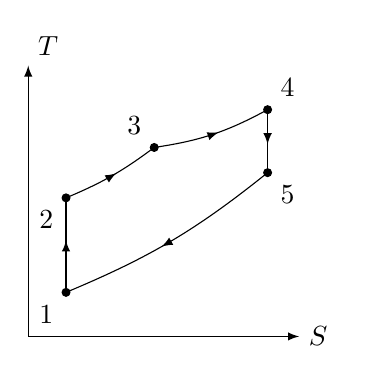
\begin{tikzpicture}[
	scale=0.8, every node/.style={scale=1},
  > = latex,
  dot/.style = {draw,fill,circle,inner sep=1pt},
  arrow inside/.style = {postaction=decorate,decoration={markings,mark=at position .55 with \arrow{>}}}
  ]
  	\draw[<->] (0,4.3) node[above right] {$T$} |- (4.3,0) node[right] {$S$};

	\coordinate (@1) at (0.6,0.7);
	\coordinate (@2) at (0.6,2.2);
	\coordinate (@3) at (2,3);
	\coordinate (@4) at (3.8,3.6);
	\coordinate (@5) at (3.8,2.6);

	\node[dot,label={below left:$1$}] at (@1) {};
	\node[dot,label={below left:$2$}] at (@2) {};
	\node[dot,label={above left:$3$}] at (@3) {};
	\node[dot,label={above right:$4$}] at (@4) {};
	\node[dot,label={below right:$5$}] at (@5) {};

  	\draw[arrow inside] (@1) to (@2);
	\draw[arrow inside] (@2) to[bend right=7] (@3);
	\draw[arrow inside] (@3) to[bend right=10] (@4);
  	\draw[arrow inside] (@4) to (@5);
	\draw[arrow inside] (@5) to[bend left=8] (@1);

\end{tikzpicture}
		&
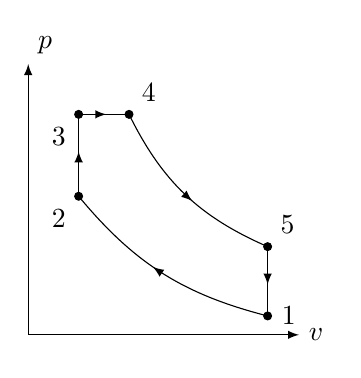
\begin{tikzpicture}[
	scale=0.8, every node/.style={scale=1},
  > = latex,
  dot/.style = {draw,fill,circle,inner sep=1pt},
  arrow inside/.style = {postaction=decorate,decoration={markings,mark=at position .55 with \arrow{>}}}
  ]
	\draw[<->] (0,4.3) node[above right] {$p$} |- (4.3,0) node[right] {$v$};

	\coordinate (@1) at (3.8,0.3);
	\coordinate (@2) at (0.8,2.2);
	\coordinate (@3) at (0.8,3.5);
	\coordinate (@4) at (1.6,3.5);
	\coordinate (@5) at (3.8,1.4);

	\node[dot,label={right:$1$}] at (@1) {};
	\node[dot,label={below left:$2$}] at (@2) {};
	\node[dot,label={below left:$3$}] at (@3) {};
	\node[dot,label={above right:$4$}] at (@4) {};
	\node[dot,label={above right:$5$}] at (@5) {};

	\draw[arrow inside] (@1) to[bend left=18] (@2);
  	\draw[arrow inside] (@2) to (@3);
  	\draw[arrow inside] (@3) to (@4);
	\draw[arrow inside] (@4) to[bend right=20] (@5);
  	\draw[arrow inside] (@5) to (@1);

\end{tikzpicture} & 
	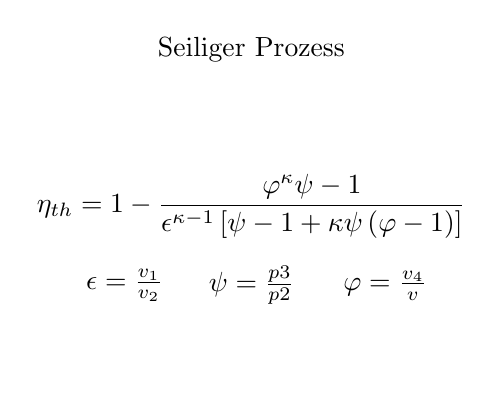
\begin{tikzpicture}
		\draw (1,4) node {Seiliger Prozess};
		\draw (1,2) node {$\displaystyle	\eta_{th} = 1 - \frac{\varphi^\kappa \psi - 1}{\epsilon^{\kappa-1}\left[\psi - 1 + \kappa \psi \left(\varphi -1 \right)\right]}$ };
		\draw (0,1) node[left] {$\epsilon = \frac{v_1}{v_2} $};
		\draw (1,1) node {$\psi     = \frac{p3}{p2}   $};
		\draw (2.7,1) node {$\varphi  = \frac{v_4}{v}   $};
		\draw (1,0);
	\end{tikzpicture}
\\ \hline
%\subsection{Otto-Prozess}

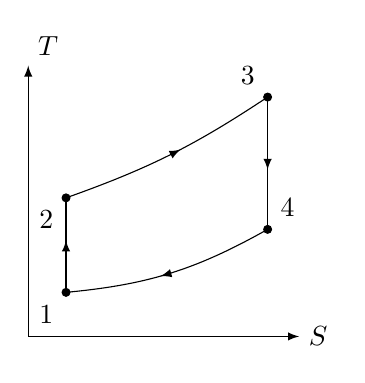
\begin{tikzpicture}[
	scale=0.8, every node/.style={scale=1},
  > = latex,
  dot/.style = {draw,fill,circle,inner sep=1pt},
  arrow inside/.style = {postaction=decorate,decoration={markings,mark=at position .55 with \arrow{>}}}
  ]
  	\draw[<->] (0,4.3) node[above right] {$T$} |- (4.3,0) node[right] {$S$};

	\coordinate (@1) at (0.6,0.7);
	\coordinate (@2) at (0.6,2.2);
	\coordinate (@3) at (3.8,3.8);
	\coordinate (@4) at (3.8,1.7);

	\node[dot,label={below left:$1$}] at (@1) {};
	\node[dot,label={below left:$2$}] at (@2) {};
	\node[dot,label={above left:$3$}] at (@3) {};
	\node[dot,label={above right:$4$}] at (@4) {};

  	\draw[arrow inside] (@1) to (@2);
	\draw[arrow inside] (@2) to[bend right=7] (@3);
	\draw[arrow inside] (@3) to (@4);
	\draw[arrow inside] (@4) to[bend left=12] (@1);

\end{tikzpicture}
&
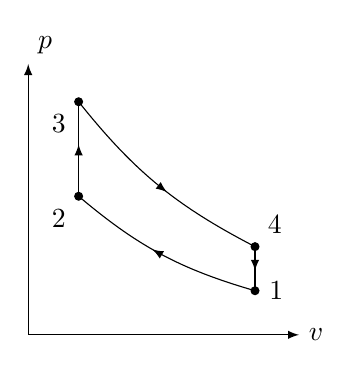
\begin{tikzpicture}[
	scale=0.8, every node/.style={scale=1},
  > = latex,
  dot/.style = {draw,fill,circle,inner sep=1pt},
  arrow inside/.style = {postaction=decorate,decoration={markings,mark=at position .55 with \arrow{>}}}
  ]
	\draw[<->] (0,4.3) node[above right] {$p$} |- (4.3,0) node[right] {$v$};

	\coordinate (@1) at (3.6,0.7);
	\coordinate (@2) at (0.8,2.2);
	\coordinate (@3) at (0.8,3.7);
	\coordinate (@4) at (3.6,1.4);

	\node[dot,label={right:$1$}] at (@1) {};
	\node[dot,label={below left:$2$}] at (@2) {};
	\node[dot,label={below left:$3$}] at (@3) {};
	\node[dot,label={above right:$4$}] at (@4) {};

	\draw[arrow inside] (@1) to[bend left=12] (@2);
  	\draw[arrow inside] (@2) to (@3);
	\draw[arrow inside] (@3) to[bend right=12] (@4);
	\draw[arrow inside] (@4) to (@1);

\end{tikzpicture}
&
	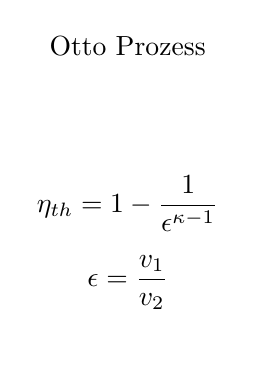
\begin{tikzpicture}
		\draw (1,4) node {Otto Prozess};
		\draw (1,2) node {$\displaystyle \eta_{th} = 1 -\frac{1}{\epsilon^{\kappa  -1}} $};
		\draw (1,1) node { $\displaystyle \epsilon 	= \frac{v_1}{v_2} $ };
		\draw (1,0);
	\end{tikzpicture}

\\ \hline

%\subsection{Diesel-Prozess}

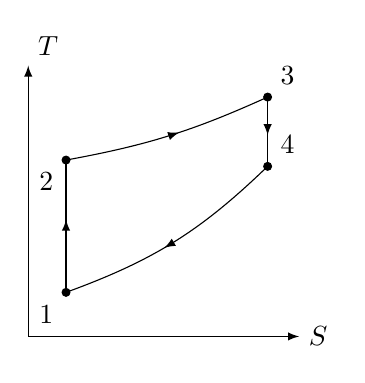
\begin{tikzpicture}[
	scale=0.8, every node/.style={scale=1},
  > = latex,
  dot/.style = {draw,fill,circle,inner sep=1pt},
  arrow inside/.style = {postaction=decorate,decoration={markings,mark=at position .55 with \arrow{>}}}
  ]
  	\draw[<->] (0,4.3) node[above right] {$T$} |- (4.3,0) node[right] {$S$};

	\coordinate (@1) at (0.6,0.7);
	\coordinate (@2) at (0.6,2.8);
	\coordinate (@3) at (3.8,3.8);
	\coordinate (@4) at (3.8,2.7);

	\node[dot,label={below left:$1$}] at (@1) {};
	\node[dot,label={below left:$2$}] at (@2) {};
	\node[dot,label={above right:$3$}] at (@3) {};
	\node[dot,label={above right:$4$}] at (@4) {};

  	\draw[arrow inside] (@1) to (@2);
	\draw[arrow inside] (@2) to[bend right=7] (@3);
	\draw[arrow inside] (@3) to (@4);
	\draw[arrow inside] (@4) to[bend left=12] (@1);

\end{tikzpicture}
&
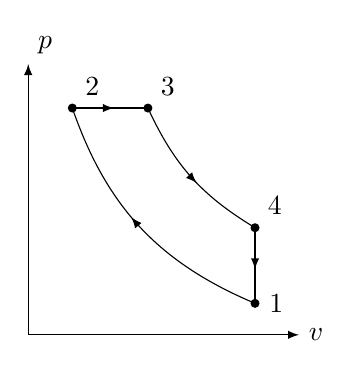
\begin{tikzpicture}[
	scale=0.8, every node/.style={scale=1},
  > = latex,
  dot/.style = {draw,fill,circle,inner sep=1pt},
  arrow inside/.style = {postaction=decorate,decoration={markings,mark=at position .55 with \arrow{>}}}
  ]
	\draw[<->] (0,4.3) node[above right] {$p$} |- (4.3,0) node[right] {$v$};

	\coordinate (@1) at (3.6,0.5);
	\coordinate (@2) at (0.7,3.6);
	\coordinate (@3) at (1.9,3.6);
	\coordinate (@4) at (3.6,1.7);

	\node[dot,label={right:$1$}] at (@1) {};
	\node[dot,label={above right:$2$}] at (@2) {};
	\node[dot,label={above right:$3$}] at (@3) {};
	\node[dot,label={above right:$4$}] at (@4) {};

	\draw[arrow inside] (@1) to[bend left=24] (@2);
  	\draw[arrow inside] (@2) to (@3);
	\draw[arrow inside] (@3) to[bend right=17] (@4);
	\draw[arrow inside] (@4) to (@1);

\end{tikzpicture}
&

	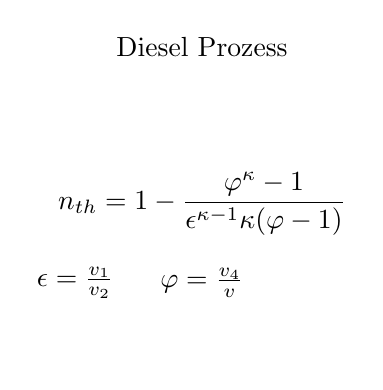
\begin{tikzpicture}
		\draw (1,4) node {Diesel Prozess};
		\draw (1,2) node {$\displaystyle	n_{th} = 1 - \frac{\varphi^\kappa - 1}{\epsilon^{\kappa -1}\kappa(\varphi - 1)}$};
		\draw (0,1) node[left] {$\epsilon = \frac{v_1}{v_2} $};
		\draw (1,1) node {$\varphi  = \frac{v_4}{v}   $};
		\draw (1,0);
	\end{tikzpicture}
\\ \hline
%\subsection{Stirling-Prozess}

\begin{tikzpicture}[
	scale=0.8, every node/.style={scale=1},
  > = latex,
  dot/.style = {draw,fill,circle,inner sep=1pt},
  arrow inside/.style = {postaction=decorate,decoration={markings,mark=at position .55 with \arrow{>}}}
  ]
  	\draw[<->] (0,4.3) node[above right] {$T$} |- (4.3,0) node[right] {$S$};

	\coordinate (@1) at (2.8,1);
	\coordinate (@2) at (0.5,1);
	\coordinate (@3) at (2.0,3.3);
	\coordinate (@4) at (4,3.3);

	\node[dot,label={below left:$1$}] at (@1) {};
	\node[dot,label={below left:$2$}] at (@2) {};
	\node[dot,label={above right:$3$}] at (@3) {};
	\node[dot,label={above right:$4$}] at (@4) {};

  	\draw[arrow inside] (@1) to (@2);
	\draw[arrow inside] (@2) to[bend right=7] (@3);
	\draw[arrow inside] (@3) to (@4);
	\draw[arrow inside] (@4) to[bend left=12] (@1);

\end{tikzpicture}
&
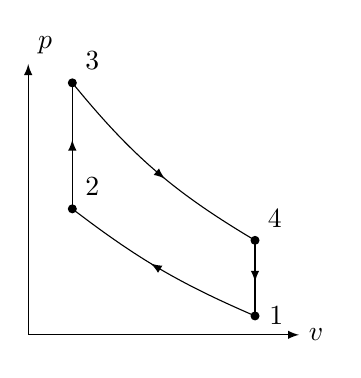
\begin{tikzpicture}[
	scale=0.8, every node/.style={scale=1},
  > = latex,
  dot/.style = {draw,fill,circle,inner sep=1pt},
  arrow inside/.style = {postaction=decorate,decoration={markings,mark=at position .55 with \arrow{>}}}
  ]
	\draw[<->] (0,4.3) node[above right] {$p$} |- (4.3,0) node[right] {$v$};

	\coordinate (@1) at (3.6,0.3);
	\coordinate (@2) at (0.7,2.0);
	\coordinate (@3) at (0.7,4);
	\coordinate (@4) at (3.6,1.5);

	\node[dot,label={right:$1$}] at (@1) {};
	\node[dot,label={above right:$2$}] at (@2) {};
	\node[dot,label={above right:$3$}] at (@3) {};
	\node[dot,label={above right:$4$}] at (@4) {};

	\draw[arrow inside] (@1) to[bend left=7] (@2);
  	\draw[arrow inside] (@2) to (@3);
	\draw[arrow inside] (@3) to[bend right=10] (@4);
	\draw[arrow inside] (@4) to (@1);

\end{tikzpicture}
&

	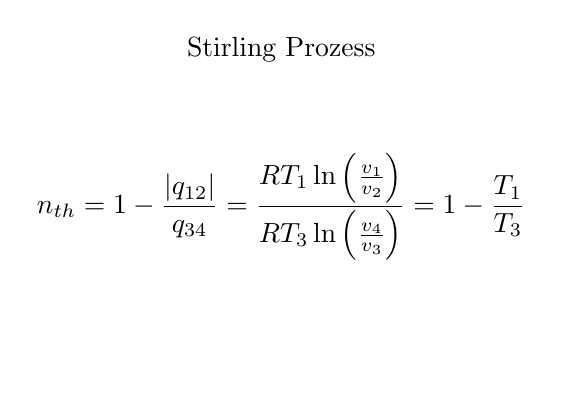
\begin{tikzpicture}
		\draw (1,4) node {Stirling Prozess};
		\draw (1,2) node {$\displaystyle	n_{th} = 1 - \frac{|q_{12}|}{q_{34}} = \frac{RT_1 \ln\left(\frac{v_1}{v_2}\right)}{RT_3 \ln \left(\frac{v_4}{v_3}\right)}= 1 - \frac{T_1}{T_3}$};
		\draw (1,0);
\end{tikzpicture}  
\\ \hline
%\subsection{Joule-Prozess}


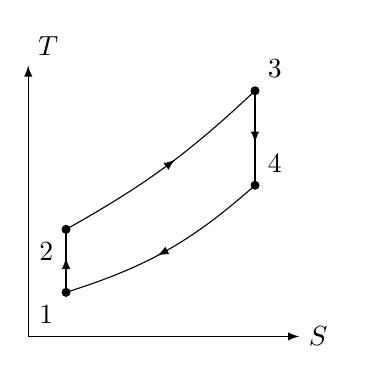
\begin{tikzpicture}[
	scale=0.8, every node/.style={scale=1},
  > = latex,
  dot/.style = {draw,fill,circle,inner sep=1pt},
  arrow inside/.style = {postaction=decorate,decoration={markings,mark=at position .55 with \arrow{>}}}
  ]
  	\draw[<->] (0,4.3) node[above right] {$T$} |- (4.3,0) node[right] {$S$};

	\coordinate (@1) at (0.6,0.7);
	\coordinate (@2) at (0.6,1.7);
	\coordinate (@3) at (3.6,3.9);
	\coordinate (@4) at (3.6,2.4);

	\node[dot,label={below left:$1$}] at (@1) {};
	\node[dot,label={below left:$2$}] at (@2) {};
	\node[dot,label={above right:$3$}] at (@3) {};
	\node[dot,label={above right:$4$}] at (@4) {};

  	\draw[arrow inside] (@1) to (@2);
	\draw[arrow inside] (@2) to[bend right=7] (@3);
	\draw[arrow inside] (@3) to (@4);
	\draw[arrow inside] (@4) to[bend left=12] (@1);

\end{tikzpicture}
&
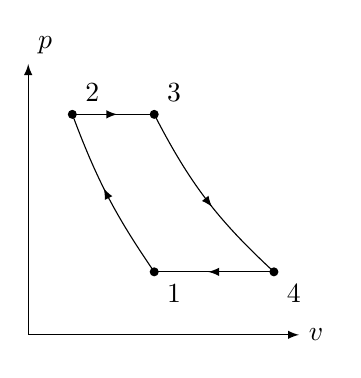
\begin{tikzpicture}[
	scale=0.8, every node/.style={scale=1},
  > = latex,
  dot/.style = {draw,fill,circle,inner sep=1pt},
  arrow inside/.style = {postaction=decorate,decoration={markings,mark=at position .55 with \arrow{>}}}
  ]
	\draw[<->] (0,4.3) node[above right] {$p$} |- (4.3,0) node[right] {$v$};

	\coordinate (@1) at (2,1);
	\coordinate (@2) at (0.7,3.5);
	\coordinate (@3) at (2,3.5);
	\coordinate (@4) at (3.9,1);

	\node[dot,label={below right:$1$}] at (@1) {};
	\node[dot,label={above right:$2$}] at (@2) {};
	\node[dot,label={above right:$3$}] at (@3) {};
	\node[dot,label={below right:$4$}] at (@4) {};

	\draw[arrow inside] (@1) to[bend left=7] (@2);
  	\draw[arrow inside] (@2) to (@3);
	\draw[arrow inside] (@3) to[bend right=10] (@4);
	\draw[arrow inside] (@4) to (@1);

\end{tikzpicture}
&

	\begin{tikzpicture}
		\draw (1,4) node {Joule Prozess};
		\draw (1,2) node {$\displaystyle \eta_{th} = 1 - \frac{T_1}{T_2} = 1 - \left(\frac{p_1}{p_2}\right)^{\frac{\kappa-1}{\kappa}} = 1 - \left( \frac{1}{\pi}\right)^{\frac{\kappa -1 }{\kappa}}$};
		\draw (1,1) node {$\pi = \frac{p_2}{p_1}$};
		\draw (1,0);
	\end{tikzpicture}
\\ \hline
%\subsection{Ericsson-Prozess}

\begin{tikzpicture}[
	scale=0.8, every node/.style={scale=1},
  > = latex,
  dot/.style = {draw,fill,circle,inner sep=1pt},
  arrow inside/.style = {postaction=decorate,decoration={markings,mark=at position .55 with \arrow{>}}}
  ]
  	\draw[<->] (0,4.3) node[above right] {$T$} |- (4.3,0) node[right] {$S$};

	\coordinate (@1) at (2.8,1);
	\coordinate (@2) at (0.5,1);
	\coordinate (@3) at (2.0,3.3);
	\coordinate (@4) at (4,3.3);

	\node[dot,label={below left:$1$}] at (@1) {};
	\node[dot,label={below left:$2$}] at (@2) {};
	\node[dot,label={above right:$3$}] at (@3) {};
	\node[dot,label={above right:$4$}] at (@4) {};

  	\draw[arrow inside] (@1) to (@2);
	\draw[arrow inside] (@2) to[bend right=7] (@3);
	\draw[arrow inside] (@3) to (@4);
	\draw[arrow inside] (@4) to[bend left=12] (@1);

\end{tikzpicture}
&
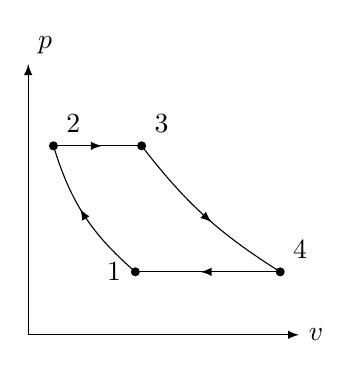
\begin{tikzpicture}[
	scale=0.8, every node/.style={scale=1},
  > = latex,
  dot/.style = {draw,fill,circle,inner sep=1pt},
  arrow inside/.style = {postaction=decorate,decoration={markings,mark=at position .55 with \arrow{>}}}
  ]
	\draw[<->] (0,4.3) node[above right] {$p$} |- (4.3,0) node[right] {$v$};

	\coordinate (@1) at (1.7,1);
	\coordinate (@2) at (0.4,3.0);
	\coordinate (@3) at (1.8,3);
	\coordinate (@4) at (4,1);

	\node[dot,label={left:$1$}] at (@1) {};
	\node[dot,label={above right:$2$}] at (@2) {};
	\node[dot,label={above right:$3$}] at (@3) {};
	\node[dot,label={above right:$4$}] at (@4) {};

	\draw[arrow inside] (@1) to[bend left=16] (@2);
  	\draw[arrow inside] (@2) to (@3);
	\draw[arrow inside] (@3) to[bend right=10] (@4);
	\draw[arrow inside] (@4) to (@1);

\end{tikzpicture}
&

	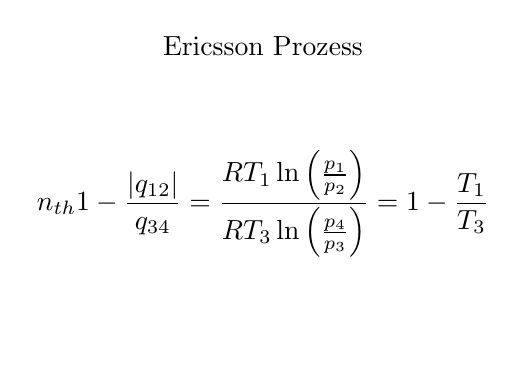
\begin{tikzpicture}
		\draw (1,4) node {Ericsson Prozess};
		\draw (1,2) node {$\displaystyle	n_{th} 1 - \frac{|q_{12}|}{q_{34}} = \frac{RT_1 \ln\left(\frac{p_1}{p_2}\right)}{RT_3 \ln \left(\frac{p_4}{p_3}\right)}= 1 - \frac{T_1}{T_3}$};
		\draw (1,0);
\end{tikzpicture}  
\end{tabular}
\end{table}

\onecolumn

%       ____    __           __             ______              
%      /  _/___/ /__  ____ _/ /__  _____   / ____/___ ______    
%      / // __  / _ \/ __ `/ / _ \/ ___/  / / __/ __ `/ ___/    
%    _/ // /_/ /  __/ /_/ / /  __(__  )  / /_/ / /_/ (__  )     
%   /___/\__,_/\___/\__,_/_/\___/____/   \____/\__,_/____/      
                                                               
\begin{landscape}
	\LARGE
	Ideales Gas 
	\\\\
	\renewcommand{\arraystretch}{2}
\begin{tabular}{l|l|l|l|l|l}
& Isothermo  
& Isobare  
& Isochore  
& Isentrop  
& Polytrope 
\\ \hline
  konstant:  
& T  
& p  
& v  
& $\delta q=0$  
& $pv^n$  
\\ \hline
	
& -  
& -  
& -  
& $p_1 v_1^{\kappa} = p_2 v_2^{\kappa}$  
& $v_1^{n} = p_2 v_2^{n}$  
\\ \hline

& $p_1 p_2 = p_2 v_2$  
& $\frac{v_1}{v_2} = \frac{T_1}{T_2}$  
& $\frac{p_1}{T_1} = \frac{p_2}{T_2}$  
& $T_1 v_1^{\kappa - 1} = T_2 v_2^{\kappa -1}$   
& $T_1 v_1^{n - 1} = T_2 v_2^{n -1}$  
\\ \hline
	
& -  
& -  
& $\small\xrightswishingghost{}$  
& $\frac{T_1^{\frac{\kappa}{\kappa -1}}}{p_1} = \frac{T_2^{\frac{\kappa}{\kappa -1}}}{p_2}$  
& $\frac{T_1^{\frac{n}{n -1}}}{p_1} = \frac{T_2^{\frac{n}{n -1}}}{p_2}$  
\\ \hline

	$p,v$

& $p = \frac{p_1 v_1}{v}$  
& $p = p_1$  
& $v = v_1$  
& $p = \frac{p_1 v_1^{\kappa}}{v^{\kappa}}$  
& $p = \frac{p_1 v_1^{n}}{v^{n}}$ 
\\ \hline

	$p,T$

& $p = \frac{p_1 v_1}{v}$  
& $p = p_1$  
& $p = \frac{p_1}{T_1}T$  
& $p = \frac{p_1}{T_1^{\frac{\kappa}{\kappa -1}}} T^{\frac{\kappa}{\kappa -1}}$  
& $p = \frac{p_1}{T_1^{\frac{n}{n -1}}} T^{\frac{n}{n -1}}$
\\ \hline

	$v,T$  

& $T = T_1$  
& $v = \frac{v_1}{T_1}T$  
& $v = v_1 $ 
& $T = \frac{T_1 v_1^{\kappa - 1}}{v^{\kappa - 1}}$  
& $T = \frac{T_1v_1^{n-1}}{v^{n-1}}  $
\\ \hline

	$q_{12}$	

& $= p_1v_1 \ln \frac{p_1}{p_2}$  
& $= c_p(T_2 - T_1)$   
& $= c_v(T_2 - T_1)$  
& $= 0$   
&  $= c_v \frac{n-\kappa}{n-1}(T_2-T_1)$ 
\\ \hline

	$w_{V,12}$  

& $= -q_{12}$ 
& $= -p_1(v_2 - v_1)$  
& $= 0$  
& $= \frac{p_1 v_1}{k - 1}\left[\left(\frac{v_1}{v_1}\right)^{\kappa - 1} - 1\right]$  
& $= \frac{p_1 v_1}{n - 1}\left[\left(\frac{v_1}{v_2}\right)^{n-1} - 1\right]$ 
\\ \hline

	$s_2 - s_1$ 

& $= R \ln \left(\frac{p_1}{p_2}\right)$  
& $= c_p \ln \left(\frac{T_2}{T_1}\right)$  
& $= c_v \ln \left(\frac{T_2}{T_1}\right)$  
& $= 0$  
& $= c_v \frac{n - \kappa }{n - 1} \ln \left(\frac{T_2}{T_1}\right)$  
\\ 
\end{tabular}
\bigskip
\\\\
% _    __                  ____                _       __            __         
%| |  / /___ _____        / __ \___  _____    | |     / /___ _____ _/ /____     
%| | / / __ `/ __ \______/ / / / _ \/ ___/____| | /| / / __ `/ __ `/ / ___/_____
%| |/ / /_/ / / / /_____/ /_/ /  __/ /  /_____/ |/ |/ / /_/ / /_/ / (__  )_____/
%|___/\__,_/_/ /_/     /_____/\___/_/         |__/|__/\__,_/\__,_/_/____/       
%                                                                               
%   ______                
%  / ____/___ ______      
% / / __/ __ `/ ___/      
%/ /_/ / /_/ (__  )       
%\____/\__,_/____/        

\Large
Van-Der-Waals-Gas  
\\

	\begin{tabular}{l|l|l|l|l}
		
& Isotherme 
& Isobare 
& Isochore 
& Isentrop 
\\ \hline
		konst. 
& T 
& p 
& v  
& $\delta = 0$ 
\\ \hline
		
& \thead{\Large$(p_1 + \frac{a}{v^2})(v_1-b)$ \\\Large $= (p_2 + \frac{a}{v^2})(v_2-b)$}
& \Large$\frac{RT_1}{v_1-b} - \frac{a}{v_1^2} = \frac{RT_2}{v-b} - \frac{a}{v_2^2}$ 
& $\frac{p_1 + \frac{a}{v_1^2}}{T_1} = \frac{p_2 + \frac{a}{v_1^2}}{T_2}$  
& \thead{\large $(p_1 + \frac{a}{v^2}) (v_1-b)^{\frac{c_v + R}{c_v}}$ \\\large $ = (p + \frac{a}{v^2}) (v_2-b)^{\frac{c_v + R}{c_v}},$ \\ \large $ \quad T_1(v_1-b)^{R/c_v} = T_2 (v_2-b)^{R/c_v}$}  
\\ \hline

		$p,v$ 

& $p = (p + \frac{a}{v^2}) \frac{v_u}{v-b} - \frac{a}{v^2}$ 
& $p = p_1$  
& $v = v_1$ 
& $p = - \frac{a}{v^2} + (p_1 + \frac{a}{v^2}) \left(\frac{v_1-b}{v_m}\right)^{\frac{v_v + R }{R}}$ 
\\ \hline

		$p,T$ 

& $T = T_1$ 
& $p = p_1$ 
& $p = \frac{T}{T_1} (p_1 + \frac{a}{v^2}) - \frac{a}{v_1^2}$ 
& $p = - \frac{a}{v^2}+ (p_1 + \frac{a}{v^2}) \left(\frac{T}{T_1}\right)^\frac{c_v+R}{R}$ 
\\ \hline

		$v,T$ 

& $T = T_1$ 
& $T = T_1 \frac{v-b}{v_1-b} + \frac{a}{R}(v-b) \left(\frac{1}{v^2} - \frac{1}{v_1^2}\right)$ 
& $v = v_1$  
& $T = T_1 \left(\frac{v_1-b}{v-b}\right)^\frac{R}{c_v}$ 
\\ \hline

		$q_{12}$ 

& $= RT_1 \ln \left(\frac{v_2-b}{v_1-b}\right)$ 
& $= \frac{a}{v_1} - \frac{a}{v_2} + c_v(T_2 - T_1) + p_1(v_2 - v_1)$ 
& $= c_v(T_2 - T_1)$  
& $= 0$  
\\ \hline

		$w_{V,12}$ 

& $= -RT_1 \ln \left(\frac{v_2-b}{v_1-b}\right) + \frac{a}{v_1} - \frac{a}{v_2}$ 
& $= -p_1(v_2-v_1)$ 
& $= 0$  
& $= \frac{a}{v_1} - \frac{a}{v_2} + c_v(T_2 - T_1)$ 
\\ \hline

		$s_2 - s_1$ 

& $= R\ln \left(\frac{v_2-b}{v_1-b}\right)$ 
& $= c_v \ln \left(\frac{T_2}{T_1}\right) + R \ln \left(\frac{v_2-b}{v_1-b}\right)$ 
& $= c_v \ln \left(\frac{T_2}{T_1}\right)$ 
& $= 0$ 
\\
\end{tabular}
\end{landscape}

%   _____ __        ________                   __     
%  / ___// /_____  / __/ __/      _____  _____/ /____ 
%  \__ \/ __/ __ \/ /_/ /_| | /| / / _ \/ ___/ __/ _ \
% ___/ / /_/ /_/ / __/ __/| |/ |/ /  __/ /  / /_/  __/
%/____/\__/\____/_/ /_/   |__/|__/\___/_/   \__/\___/ 
%	                                                     
%    _______       _                    ______              
%   / ____(_)___  (_)___ ____  _____   / ____/___ _________ 
%  / __/ / / __ \/ / __ `/ _ \/ ___/  / / __/ __ `/ ___/ _ \
% / /___/ / / / / / /_/ /  __/ /     / /_/ / /_/ (__  )  __/
%/_____/_/_/ /_/_/\__, /\___/_/      \____/\__,_/____/\___/ 
%                /____/                                     
%
\section{Stoffwerte einiger Gase}

\begin{center}

\begin{tabular}{l|l|r|r|r|r|r|r}
Bezeichnung	&	Symbol	&Molmasse 	&Gaskonstante	&	Dichte	& $c_p$ & $c_v$ &$\kappa$ \\
		&		&[kg/kmol]	&[J/(kg K)]	& 	[kg/m3]	& [J/(kg K)]	& [J/(kg,K)] & \\
	&&&&&&\\
Acetylen	&$	C_2H_2	$&	26.038	&	319.3	&	1.16 	&	1616	&	1278	&	1.26 \\
Ammoniak	&$	NH_3	$&	17.031	&	488.2	&	0.76 	&	2056	&	1526	&	1.35 \\
Argon		&$	Ar	$&	39.948	&	208.1	&	1.76 	&	519	&	309	&	1.68 \\
Äthan		&$	C_2H_6	$&	30.070	&	276.5	&	1.34 	&	1650	&	1355	&	1.22 \\
Butan		&$	C_4H_10	$&	58.124	&	143.0	&	2.67 	&	1599	&	1410	&	1.13 \\
Chlor		&$	C_l2	$&	56.108	&	117.3	&	3.17 	&	473	&	343	&	1.38 \\
Chlorwasserstoff&$	HCl	$&	70.906	&	228.0	&	1.62 	&	795	&	556	&	1.43 \\
Helium		&$	He	$&	4.003	&	2077.0	&	0.18 	&	5200	&	3124	&	1.66 \\
Kohlendioxid	&$	CO_2	$&	44.010	&	188.9	&	1.95 	&	816	&	618	&	1.32 \\
Kohlenmonoxid	&$	CO	$&	28.010	&	296.8	&	1.23 	&	1038	&	739	&	1.40 \\
Luft		&$	–	$&	28.964	&	287.1	&	1.28 	&	1006	&	718	&	1.40 \\
Methan		&$	CH_4	$&	16.043	&	518.3	&	0.71 	&	2165	&	1638	&	1.32 \\
Propan		&$	C_3H_8	$&	44.097	&	188.5	&	1.99 	&	1549	&	1331	&	1.16 \\
Sauerstoff	&$	O_2	$&	31.999	&	259.8	&	1.41 	&	909	&	647	&	1.40 \\
Stickstoff	&$	N_2	$&	28.013	&	296.8	&	1.23 	&	1038	&	739	&	1.40 \\
Wasserstoff	&$	H_2	$&	2.016	&	4124.2	&	0.09 	&	14050	&	9926	&	1.42 \\
Xenon		&$	Xe	$&	131.300	&	63.3	&	5.82 	&	159	&	93	&	1.71 \\
\end{tabular}

\end{center}
%   _____ __        ________    __      __                     _       _                
%  / ___// /_____  / __/ __/___/ /___ _/ /____  ____     ___  (_)___  (_)___ ____  _____
%  \__ \/ __/ __ \/ /_/ /_/ __  / __ `/ __/ _ \/ __ \   / _ \/ / __ \/ / __ `/ _ \/ ___/
% ___/ / /_/ /_/ / __/ __/ /_/ / /_/ / /_/  __/ / / /  /  __/ / / / / / /_/ /  __/ /    
%/____/\__/\____/_/ /_/  \__,_/\__,_/\__/\___/_/ /_/   \___/_/_/ /_/_/\__, /\___/_/     
%                                                                    /____/             
%   _____ __        ________   
%  / ___// /_____  / __/ __/__ 
%  \__ \/ __/ __ \/ /_/ /_/ _ \
% ___/ / /_/ /_/ / __/ __/  __/
%/____/\__/\____/_/ /_/  \___/ 
%										                                  
%
\section{Stoffdaten einiger Stoffe}

\begin{center}

\begin{tabular}{l|r|r|r|r|r}
	Name	& chemische &	 Molmasse  	& Normal-& kritische & kritischer \\
Name	& Formel&	 [kg/kmol]	& siedepunkt [\textcelsius]	& Temperatur [\textcelsius]	& Druck [MPa] 	\\
		&			&			&			&		&	 	\\
Wasserstoff	&	$H_2$		&		2.02	&		-252.9	&	-240.0	&	1.32 	\\
Helium		&	$He$		&		4.00	&		-268.9	&	-268.0	&	0.23 	\\
Ammoniak	&	$NH_3$		&		17.03	&		-33.3	&	132.3	&	11.33 	\\
Wasser		&	$H_2O$		&		18.02	&		100.0	&	373.9	&	22.06 	\\
Luft		&\begin{tabular}{r} $78\%$ 	\\ $N_2 21\%$ \\ $O_2. 1\% Ar.+$\end{tabular}&	28.96	&	-194.2	&-140.4	&3.84 \\
Kohlendioxid	&	$CO_2$		&		44.01	&		-78.4	&	31.0	&	7.38 	\\
Methan		&	$CH_4$		&		16.04	&		-161.5	&	-82.6	&	4.60 	\\
Äthan		&	$C_2H_6$	&		30.07	&		-88.6	&	32.2	&	4.87 	\\
Propan		&	$C_3H_8$	&		44.10	&		-42.1	&	96.7	&	4.25 	\\
R134a		&	$CH_2FCF_3$	&		102.03	&		-26.1	&	101.1	&	4.06 	\\
\end{tabular}

\end{center}

%   ____  __         __                 
%  / __ \/ /_  _____/ /____  __________ 
% / / / / __ \/ ___/ //_/ / / / ___/ _ \
%/ /_/ / /_/ (__  ) ,< / /_/ / /  /  __/
%\____/_.___/____/_/|_|\__,_/_/   \___/ 
%                                             
% _____                                                   __     /\// /|___/|              
%/__  /  __  ___________ _____ ___  ____ ___  ___  ____  / /_  _//\/ | __  /___  ____ ____ 
%  / /  / / / / ___/ __ `/ __ `__ \/ __ `__ \/ _ \/ __ \/ __ \/ _ | / /_/ / __ \/ __ `/ _ \
% / /__/ /_/ (__  ) /_/ / / / / / / / / / / /  __/ / / / / / / __ |/___  / / / / /_/ /  __/
%/____/\__,_/____/\__,_/_/ /_/ /_/_/ /_/ /_/\___/_/ /_/_/ /_/_/ |_|/   |/_/ /_/\__, /\___/ 
%                                                                             /____/       
%
\section{Obskure Zusammenhänge}



\begin{align*}
	dV	&= \left(\frac{\partial V}{\partial T}\right)_{p} dT 
	+ \left(\frac{\partial V}{\partial p}\right)_{T,n}  
	+ \sum_{k=1}^{K} \left(\frac{\partial V}{\partial n_k}\right)_{T,p} dkn_k \\
	dS	&= \left(\frac{nC_{p,m}}{T} \right) dT 
	- \left(\frac{\partial V}{\partial T}\right)_{p,n} dp 
	+ \sum_{k=1}^{K} \left(\frac{\partial \mu_k}{\partial T}\right)_{p,n} dn_k \\
	dU	&= \left[nC_{p,m} 
	- p \left(\frac{\partial V}{\partial T}\right)_{p,n}\right]dT 
	-  \left[p\left(\frac{\partial V}{\partial p}\right)_{T,n} 
	+ T \left(\frac{\partial V}{\partial T}\right)_{p,n} \right]dp 
	+ \sum_{k=1}^{K} \left[ \mu_k 
	-T \left(\frac{\partial \mu_k}{\partial T}\right)_{p,n} 
	- p \left(\frac{\partial V}{\partial n_k}\right)_{T,p,n} \right]dn_k \\
	dH 	&= nC_{p,m} dT 
	+ \left[V T \left(\frac{\partial V}{\partial T}\right)_{p,n}\right] 
	+ \sum_{k=1}^{K} \left[ \mu_k 
	- T \left(\frac{\partial \mu_k}{\partial T}\right)_{p,n} \right] dn_k  \\
	dF	&= 
	-\left[S 
	+ p \left(\frac{\partial V}{\partial T}\right)_{p,n} \right] dT 
	- p \left(\frac{\partial V}{\partial p}\right)_{T,n} dp 
	+ \sum_{k=1}^{K} \left[\mu_k  
	- p \left(\frac{\partial V}{\partial n_k }\right)_{T,p} \right] dn_k \\
	\left(\frac{\partial C_{p,m}}{\partial p}\right)_{T,\psi_j} &= T \frac{\partial}{\partial p} \left[\left(\frac{\partial S_m }{\partial T}\right)_{p,\psi_j} \right]_{T,\psi_j} = T \frac{\partial}{\partial T}\left[ \left(\frac{\partial S_m}{\partial p}\right)_{T,\psi_j} \right]_{p,\psi_j} = 
	-T \frac{\partial}{\partial T}\left[ \left(\frac{\partial V_m}{\partial T}\right)_{p,\psi_j} \right]_{p,\psi_j} = 
	-T \left(\frac{\partial^2  V_m}{\partial T^2}\right)_{p,\psi_j} \\
	C_{p,m} &= (C_{p,m})_{\text{ideales Gas}} 
	- T \int_{0}^{p} \left(\frac{\partial^2 V_m }{\partial T^2}\right)_{p,\psi_j} \; d\tilde{p} \\
	C_{v,m} &= (C_{v,m})_{\text{ideales Gas}} 
	- T \int_{0}^{V_m} \left(\frac{\partial^2 p }{\partial T^2}\right)_{p,\psi_j} \; d\tilde{V} \\
\end{align*}
\end{document}

